%%%%%%%%%%%%%%%%%%%%%%%%%%%%%%%%%%%%%%%%%
% Short Sectioned Assignment LaTeX Template Version 1.0 (5/5/12)
% This template has been downloaded from: http://www.LaTeXTemplates.com
% Original author:  Frits Wenneker (http://www.howtotex.com)
% License: CC BY-NC-SA 3.0 (http://creativecommons.org/licenses/by-nc-sa/3.0/)
%%%%%%%%%%%%%%%%%%%%%%%%%%%%%%%%%%%%%%%%%

% \documentclass[paper=a4, fontsize=11pt]{scrartcl} % A4 paper and 11pt font size
\documentclass[11pt, a4paper,oneside]{book}
\usepackage[T1]{fontenc} % Use 8-bit encoding that has 256 glyphs
\usepackage[utf8]{inputenc}
\usepackage{fourier} % Use the Adobe Utopia font for the document - comment this line to return to the LaTeX default
\usepackage{listings} % para insertar código con formato similar al editor
\usepackage[spanish, es-tabla]{babel} % Selecciona el español para palabras introducidas automáticamente, p.ej. "septiembre" en la fecha y especifica que se use la palabra Tabla en vez de Cuadro
\usepackage{url} % ,href} %para incluir URLs e hipervínculos dentro del texto (aunque hay que instalar href)
\usepackage{graphics,graphicx, float} %para incluir imágenes y colocarlas
\usepackage[gen]{eurosym} %para incluir el símbolo del euro
\usepackage{cite} %para incluir citas del archivo <nombre>.bib
\usepackage{xcolor}
\usepackage{tcolorbox}
\tcbuselibrary{listingsutf8}
\usepackage{enumerate}
\usepackage{hyperref}
\usepackage{graphicx}
\usepackage{tabularx}
\usepackage{booktabs}
\usepackage{longtable}
\usepackage{changepage}
\usepackage{amsmath}
\usepackage{eurosym}
\usepackage[absolute,overlay]{textpos}
% Para añadir checkbox
\usepackage{enumitem,amssymb}
\usepackage{tikz}
\usetikzlibrary{shapes.geometric, arrows}
\newlist{todolist}{itemize}{2}
\setlist[todolist]{label=$\square$}
\usepackage{pifont}
\newcommand{\cmark}{\ding{51}}%
\newcommand{\xmark}{\ding{55}}%
\newcommand{\xcmark}{\rlap{$\square$}{\raisebox{2pt}{\large\hspace{1pt}\cmark}}%
\hspace{-2.5pt}}
\newcommand{\wontfix}{\rlap{$\square$}{\large\hspace{1pt}\xmark}}

\usepackage[table,xcdraw]{xcolor}
\hypersetup{
	colorlinks=true,	% false: boxed links; true: colored links
	linkcolor=black,	% color of internal links
	urlcolor=cyan		% color of external links
}
\renewcommand{\familydefault}{\sfdefault}
\usepackage{fancyhdr} % Custom headers and footers
\pagestyle{fancyplain} % Makes all pages in the document conform to the custom headers and footers
\fancyhead[L]{} % Empty left header
\fancyhead[C]{} % Empty center header
\fancyhead[R]{\nouppercase{\leftmark}} % My name
\fancyfoot[L]{} % Empty left footer
\fancyfoot[C]{} % Empty center footer
\fancyfoot[R]{\thepage} % Page numbering for right footer
%\renewcommand{\headrulewidth}{0pt} % Remove header underlines
\renewcommand{\footrulewidth}{0pt} % Remove footer underlines
\setlength{\headheight}{13.6pt} % Customize the height of the header

%Para darle estilo a las muestras de código
\definecolor{backcolour}{rgb}{0.95,0.95,0.92}
\definecolor{codegreen}{rgb}{0,0.6,0}

\usepackage{xcolor}
\usepackage{listings}
\usepackage{xurl}
\urlstyle{same}
\lstset{
  basicstyle=\ttfamily\small,
  keywordstyle=\color{blue}\bfseries,
  stringstyle=\color{teal},
  commentstyle=\color{gray}\itshape,
  identifierstyle=\color{black},
  backgroundcolor=\color{gray!10},
  frame=single,
  numbers=left,
  numberstyle=\tiny\color{gray},
  breaklines=true,
  showstringspaces=false,
}


\usepackage{titlesec, blindtext, color}
\definecolor{gray75}{gray}{0.75}
\newcommand{\hsp}{\hspace{20pt}}
\titleformat{\chapter}[hang]{\Huge\bfseries}{\thechapter\hsp\textcolor{gray75}{|}\hsp}{0pt}{\Huge\bfseries}
\setcounter{secnumdepth}{4}
\usepackage[Lenny]{fncychap}


\begin{document}

	% Plantilla portada UGR
	\begin{titlepage}
\newlength{\centeroffset}
\setlength{\centeroffset}{-0.5\oddsidemargin}
\addtolength{\centeroffset}{0.5\evensidemargin}
\thispagestyle{empty}

\noindent\hspace*{\centeroffset}\begin{minipage}{\textwidth}

\centering

\includegraphics[width=0.9\textwidth]{logos/logo_ugr.jpg}\\[1.4cm]

\textsc{ \Large TRABAJO FIN DE GRADO\\[0.2cm]}
\textsc{ GRADO EN INGENIERIA INFORMATICA}\\[1cm]

{\Huge\bfseries Sistema multiplataforma para la búsqueda y gestión de pisos compartidos \\}
\noindent\rule[-1ex]{\textwidth}{3pt}\\[3.5ex]

\end{minipage}

\vspace{1cm}
\noindent\hspace*{\centeroffset}
\begin{minipage}{\textwidth}
\centering

\textbf{Autor}\\ {Alonso Doña Martínez}\\[2.5ex]
\textbf{Director}\\ {Luis López Escudero}\\[2cm]

\includegraphics[width=0.3\textwidth]{logos/etsiit_logo.png}\\[0.1cm]
\textsc{Escuela Técnica Superior de Ingenierías Informática y de Telecomunicación}\\
\textsc{---}\\
Granada, Noviembre de 2024
\end{minipage}
\end{titlepage}


	% Plantilla prefacio UGR
	\chapter*{}

\begin{titlepage}
\newlength{\centeroffset}
\setlength{\centeroffset}{-0.5\oddsidemargin}
\addtolength{\centeroffset}{0.5\evensidemargin}
\thispagestyle{empty}


\noindent\hspace*{\centeroffset}\begin{minipage}{\textwidth}

\centering

\includegraphics[width=0.9\textwidth]{logos/logo_ugr.jpg}\\[1.4cm]

{\Huge\bfseries Sistema multiplataforma para la búsqueda y gestión de pisos compartidos \\}
\noindent\rule[-1ex]{\textwidth}{3pt}\\[3.5ex]

\end{minipage}

\vspace{1cm}
\noindent\hspace*{\centeroffset}
\begin{minipage}{\textwidth}
\centering

\textbf{Autor}\\ {Alonso Doña Martínez}\\[2.5ex]
\textbf{Director}\\ {Luis López Escudero}\\[2cm]

\end{minipage}
\end{titlepage}

\cleardoublepage
\thispagestyle{empty}
\begin{center}
{\large\bfseries Sistema multiplataforma para la búsqueda y gestión de pisos compartidos }\\
\end{center}
\begin{center}
Alonso Doña Martínez\\
\end{center}

%\vspace{0.7cm}

\vspace{0.5cm}
\noindent\textbf{Palabras clave}: \textit{Software libre}, \textit{Tecnología aplicada a la vivienda}, \textit{Co-Housing}, \textit{Gestión de pisos compartidos}, \textit{Desarrollo FullStack}
\vspace{0.7cm}

\noindent\textbf{Resumen}\\

Actualmente, uno de los principales problemas de la sociedad es la constante escalada de los precios en el ámbito de la vivienda, un desafío que afecta tanto a jóvenes como a adultos.

Una de las soluciones que está ganando terreno para mitigar los costes es la búsqueda de viviendas compartidas. Sin embargo, a pesar del contexto tecnológico actual, donde existen múltiples plataformas y portales para la búsqueda de viviendas y la organización de tareas, todos presentan limitaciones al no centrarse en ofrecer soluciones eficientes que pongan al usuario en el centro. En lugar de tratar la vivienda solo como un espacio, estas plataformas deberían considerar también los lazos y relaciones entre las personas que la habitan, brindándoles herramientas para la gestión y organización de tareas y promoviendo una convivencia agradable.

Esta \textit{plataforma}\footnote{El repositorio del proyecto está disponible en: 
\href{https://github.com/alonsodm12/TFG_COHOUSING}{Repositorio en GitHub}} nace con el objetivo de cambiar el enfoque tradicional de los pisos compartidos, creando un entorno agradable que cubra las necesidades e intereses de todos los miembros de la vivienda.

\cleardoublepage


\thispagestyle{empty}




% textidote: ignore begin %
\begin{center}
	{\large\bfseries Multiplatform system for the search and management of shared housing}\\
\end{center}
\begin{center}
	Alonso Doña Martínez\\
\end{center}
\vspace{0.5cm}
\noindent\textbf{Keywords}: \textit{Free software}, \textit{Technology applied to housing}, \textit{Co-Housing}, \textit{Shared housing management}, \textit{FullStack Development}
\vspace{0.7cm}

\noindent\textbf{Abstract}\\

Currently, one of the main problems in society is the constant rise in housing prices, a challenge that affects both young people and adults.

One of the solutions that is gaining traction to reduce costs is the search for 
shared housing. However, despite the current technological landscape, where 
multiple platforms and portals exist for finding housing and organizing tasks, 
they all have limitations as they do not focus on providing efficient and 
convenient solutions that put the user at the center. Instead of treating 
housing merely as a space, these platforms should also consider the bonds and 
relationships between the people who live there, offering them tools for task 
management and organization while promoting a pleasant coexistence.

This \textit{platform}\footnote{The repository for this project is available on GitHub: 
\href{https://github.com/alonsodm12/TFG_COHOUSING}{Github Repository}} was created with the goal of changing the traditional approach to 
shared housing, fostering an environment that aligns with the needs and 
interests of all household members.

\chapter*{}
\thispagestyle{empty}

\noindent\rule[-1ex]{\textwidth}{2pt}\\[4.5ex]

Yo, \textbf{Alonso Doña Martínez}, alumno de la titulación Ingeniería Informática de la \textbf{Escuela Técnica Superior
de Ingenierías Informática y de Telecomunicación de la Universidad de Granada}, con DNI 77555566A, autorizo la
ubicación de la siguiente copia de mi Trabajo Fin de Grado en la biblioteca del centro para que pueda ser
consultada por las personas que lo deseen.

\vspace{6cm}

\noindent Fdo: Alonso Doña Martínez

\vspace{2cm}

\begin{flushright}
Granada a 2 de Septiembre de 2025 .
\end{flushright}
\chapter*{}
\thispagestyle{empty}

\noindent\rule[-1ex]{\textwidth}{2pt}\\[4.5ex]

D. \textbf{Luis López Escudero}, Profesor del Departamento de Lenguajes y Sistemas Informáticos  de la Universidad de Granada.


\vspace{0.5cm}

\textbf{Informan:}

\vspace{0.5cm}

Que el presente trabajo, titulado \textit{\textbf{Sistema multiplataforma para la búsqueda y gestión de pisos compartidos}},
ha sido realizado bajo su supervisión por \textbf{Alonso Doña Martínez}, y autorizamos la defensa de dicho trabajo ante el tribunal
que corresponda.

\vspace{0.5cm}

Y para que conste, expiden y firman el presente informe en Granada a 2 de Septiembre de 2025 .

\vspace{1cm}

\textbf{El director:}

\vspace{5cm}

\noindent \textbf{Luis López Escudero}

\chapter*{Agradecimientos}
\thispagestyle{empty}

En primer lugar me gustaría expresar mi agradecimiento a mi tutor de TFG, Luis López Escudero, por su ayuda, compromiso y guía durante los meses de desarrollo de este proyecto.

Agradecer al personal docente de la Universidad de Granada por la dedicación y enseñanza durante estos años, claves en mi formación tanto profesional como personal.

A mi familia, por su apoyo y respaldo constante, por estar conmigo y ayudarme siempre.

A mi hermano Rafa, por ser una inspiración constante durante estos años de carrera.

A mis amigos y compañeros, por realizar este camino junto a mí, por estar en los momentos más duros, por las noches de estudio y por todas las risas.

A Carlos, por su compañerismo y amistad tanto en los momentos difíciles como bonitos de esta etapa. 

Finalmente, me gustaría agradecer a todas las personas que han permitido que el desarrollo de este proyecto haya sido posible.
\cleardoublepage

	% Índice de contenidos
	\newpage
	\tableofcontents

	% Índice de imágenes y tablas
	\newpage
	\listoffigures

	% Introducción 

	% Descripción del problema y hasta donde se llega
	

	% Estado del arte
	% 	1. Crítica al estado del arte
	% 	2. Propuesta
    \chapter{Introducción} \label{introduccion}

\section{Contexto}
En la actualidad, el acceso a la vivienda se ha convertido en un desafío tanto para jóvenes 
como adultos, especialmente en grandes ciudades donde los precios de compra y alquiler siguen 
aumentando drásticamente. 

En este contexto, ha surgido una nueva alternativa de convivencia, el 
\emph{co-housing} \cite{cohousing}, una solución innovadora que combina el acceso a una vivienda digna con el 
aprovechamiento de recursos y espacios compartidos, fomentando la colaboración y la gestión 
conjunta. Sin embargo, este modelo suele aplicarse en infraestructuras diseñadas específicamente 
para ello, lo que implica un alto coste inicial y una planificación a largo plazo.

Dado que los pisos son la forma de vivienda más extendida en las ciudades, adaptar los principios 
del \emph{co-housing} —como la búsqueda de personas afines y la vida en comunidad— a esta modalidad permitirá ofrecer una solución que mejore la calidad de vida de los individuos. Además, 
permitirá optimizar la organización de tareas y mejorar la convivencia entre los integrantes.

A pesar de sus evidentes beneficios, la gestión de pisos compartidos siguiendo estos principios presenta ciertos 
desafíos, como la organización y reparto de tareas o la búsqueda en función de la afinidad. En este sentido, la 
tecnología puede desempeñar un papel crucial en la resolución 
de estos problemas.

Este trabajo tiene como objetivo desarrollar una plataforma de creación y gestión de comunidades 
en pisos compartidos, permitiendo a los usuarios administrar estas viviendas de forma sencilla y 
moderna, fomentando un modelo de convivencia colaborativo.

\section{Motivación}
El crecimiento exponencial de las tendencias de convivencia en comunidad y el incremento del precio de la vivienda ha generado la necesidad de una plataforma tecnológica que facilite la creación, organización y administración de estos entornos en la vivienda más común: los pisos.

A pesar de la existencia de plataformas que ayudan en la búsqueda de viviendas o en la organización de tareas diarias, muchas de ellas carecen de toda la funcionalidad necesaria para aplicar los principios del \emph{co-housing}. En general, estas plataformas suelen abordar solo uno de los principios fundamentales de este tipo de convivencia, sin proporcionar una solución completa.

Teniendo esto en cuenta, la motivación de este proyecto radica en las siguientes cuestiones:

\begin{itemize}
    \item \textbf{Falta de plataformas especializadas}: Las plataformas actuales no están diseñadas para gestionar de manera completa la convivencia en pisos compartidos bajo los principios del \emph{co-housing}. Esto dificulta la implementación efectiva de este modelo de convivencia.
    
    \item \textbf{Plataforma moderna e intuitiva}: Se busca ofrecer una aplicación robusta, con una interfaz moderna y fácil de usar, que permita a los usuarios interactuar de forma sencilla y eficiente.
    
    \item \textbf{Solución a un problema actual}: El acceso a la vivienda es un desafío creciente. Según el informe del Parlamente Europeo \href{https://www.europarl.europa.eu/topics/es/article/20241014STO24542/el-aumento-del-coste-de-la-vivienda-en-la-union-europea?utm_source=chatgpt.com}{(Europarl, 2024)}, el coste de la vivienda ha aumentado significativamente en la gran mayoría de países de la Zona Euro \cite{DatosMacro}, lo que ha llevado a muchas personas a optar por viviendas compartidas como alternativa asequible. Sin embargo, la falta de herramientas adecuadas para gestionar esta convivencia puede generar conflictos y reducir la calidad de vida de los residentes.
\end{itemize}

Con base en estos puntos, este trabajo propone el desarrollo de una plataforma tecnológica que afronte estas necesidades. De esta manera, no solo se atiende una demanda real del mercado, sino que también se aplican conocimientos avanzados de ingeniería de software, siguiendo estándares de desarrollo profesional.

\section{Objetivos}
El objetivo principal de este proyecto es la creación de un sistema multiplataforma que permita la gestión de pisos compartidos, ofreciendo una respuesta moderna que aborde los principios de búsqueda por afinidad y gestión eficiente de tareas. Este objetivo se ha articulado en torno a la consecución de los siguientes objetivos:

\begin{itemize}
    \item \textbf{OE1:} Evaluar la arquitectura y tecnologías más convenientes para el problema.
    \item \textbf{OE2:} Estudiar la metodología a seguir y realizar una planificación en torno a ella.
    \item \textbf{OE3:} Utilizar \emph{GitHub} \cite{GitHub} como control de versiones e integrarlo en todo el ciclo de vida de desarrollo.
    \item \textbf{OE4:} Desarrollar una interfaz moderna e intuitiva para el usuario con tiempos de carga reducidos.
    \item \textbf{OE5:} Desarrollar la gestión de tareas que permita al usuario ver qué tiene que hacer en cada momento y qué le toca realizar a sus compañeros.
    \item \textbf{OE6:} Permitir la visualización del estado de desarrollo de las tareas.
    \item \textbf{OE7:} Desarrollar un algoritmo de recomendación que permita poner en contacto usuarios afines.
    \item \textbf{OE8:} Aprender sobre los frameworks de desarrollo \emph{Spring Boot} \cite{SpringBoot} y \emph{React} \cite{React} y ponerlos en práctica en el desarrollo del proyecto.
\end{itemize}

\section{Estructura de la memoria}
Durante el primer capítulo se han presentado tanto el contexto como la motivación para este trabajo, así como los objetivos principales que permitirán abordar el problema. El resto del contenido de la memoria se ha estructurado de la siguiente forma:

\begin{itemize}
    \item En el capítulo 2 se ha realizado una descripción del estado del arte en relación a las principales tecnologías y técnicas presentes en el mercado sobre gestión de viviendas compartidas, algoritmos de recomendación y desarrollo de aplicaciones multiplataforma.
    \item En el capítulo 3 se va a proceder a realizar ...
    \item El último capítulo aborda las conclusiones y los trabajos futuros que pueden surgir a partir de este TFG.
    \item Para finalizar, se muestran las referencias bibliográficas usadas durante la realización de este trabajo.
\end{itemize}
    \chapter{Estado del arte} \label{estado_del_arte}

\section{Análisis de las posibles soluciones al problema propuesto}
La gestión completa de pisos compartidos siguiendo los principios de convivencia propuestos por el \emph{co-housing}  plantea diversos desafíos, donde la tecnología puede ofrecer una solución efectiva que facilite su implementación.

En este contexto, es fundamental analizar y entender las soluciones tecnológicas existentes en el mercado, analizando tanto su enfoque como las herramientas utilizadas.

Para la realización de este estudio, se han analizado distintos proyectos y aplicaciones con el objetivo de identificar soluciones propuestas con anterioridad a este problema, se ha hecho especial enfoque en la usabilidad y en las herramientas utilizadas, tratando de extraer las mejores prácticas que sirvan de referencia para la creación de una solución efectiva.

\section{Revisión del estado del arte}
Para la realización de la revisión se va a seguir un esquema de temáticas, el proyecto se sustenta en dos grandes bloques: la gestion de tareas en viviendas compartidas y la búsqueda de pisos en función de afinidad entre personas. Dentro de estas dos temáticas será donde se analizarán las soluciones existentes,  buscando su aportación al enfoque de co-housing en pisos compartidos.


\subsection{Búsqueda de pisos}
\subsubsection{Idealista}
    \emph{Idealista}\cite{Idealista} es un portal inmobiliario que permite la búsqueda de pisos y habitaciones en función de criterios como la ubicación, rango de precio, aceptación de fumadores y predisposición a mascostas. Es un portal ampliamente usado, por lo que contiene un gran volumen de ofertas en distintas ciudades.
    Sin embargo, no incorpora ninguna funcionalidad que permita evaluar la afinidad entre posibles inquilinos en función de sus intereses o estilo de vida. 

\begin{figure}[H]
    \centering
    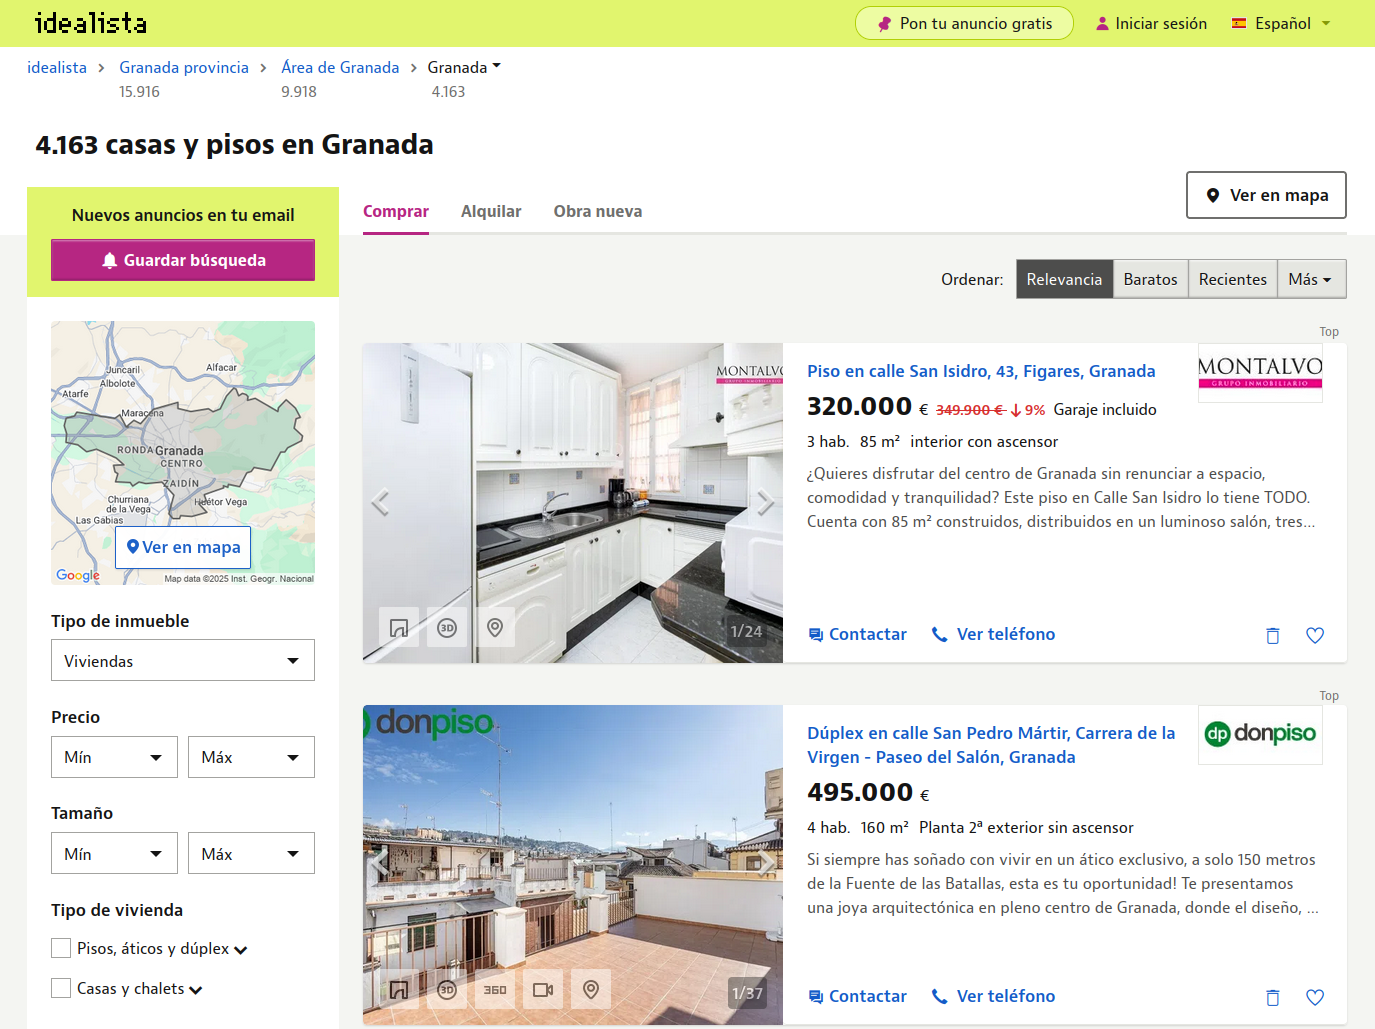
\includegraphics[width=0.8\textwidth]{fotos/idealista.png}
    \caption{Interfaz de búsqueda de Idealista\textbf{}.}
    \label{fig:idealista}
\end{figure}

\subsubsection*{Interfaz y usabilidad}
Como se puede ver en la imagen \ref{fig:idealista}, la interfaz es simple e intuitiva lo que permite que se entienda toda su funcionalidad a la perfección. Es de destacar que la aplicación te permite, con pocas configuraciones, empezar la búsqueda de piso por lo que se hace muy cómoda de usar.

\subsubsection*{Características destacadas}
\begin{itemize}
    \item \textbf{Gran volumen de ofertas:} Al ser una plataforma muy popular cuenta con un gran número de ofertas en distintas ciudades.
    \item \textbf{Filtros de búsqueda:} Permite aplicar una serie de criterios en la búsqueda como rango de precios, aceptación de fumadores, predisposición a mascotas, lo cual ayuda al usuario a encontrar un piso más acorde a sus necesidades
    \item \textbf{Comunicacion cliente-ofertante sencilla:} Facilita con su chat integrado la comunicación entre cliente y ofertante ya sea para consultar alguna duda o para realizar una reserva.
\end{itemize}
\subsubsection*{Limitaciones}
\begin{itemize}
    \item No tiene en cuenta la afinidad entre los inquilinos, lo que puede provocar que personas con diferentes intereses acaben conviviendo juntos.
    \item Se centra únicamente en la oferta de pisos, sin ofrecer ninguna herramienta para gestionar la vivienda compartida.
    \item La aplicación está orientada simplemente a encontrar potenciales inquilinos, ignorando la integración del nuevo miembro en la vivienda.
\end{itemize}

\subsubsection*{Conclusión}
\emph{Idealista} es una buena opción como portal de viviendas, ofrece posibilidades en prácticamente todas las ciudades y su facilidad de uso es correcta. Sin embargo, para la idea que buscamos es incompleta al no ofrecer nada relacionado con la búsqueda por afinidad.

\subsubsection{Flatmate Finders}
\emph{Flatmate Finders} \cite{Flatmatefinders} es una plataforma que ofrece una solución bastante precisa al problema de búsqueda de pisos por afinidad. Permitiendo al usuario dos opciones principales:

\begin{enumerate}[label=\arabic*)]
    \item \textbf{Buscar un piso}: el usuario puede crearse un perfil con información sobre su personalidad, gustos y preferencias. A partir de estos datos, la aplicación genera recomendaciones de ofertas de pisos mostrando un porcentaje de compatibilidad.
    \item \textbf{Ofrecer un piso}: los propietarios pueden registrar su vivienda, estableciendo detalles como ubicación, precio, características y criterios sobre el perfil de los inquilinos afines.
\end{enumerate}
\newpage
\begin{figure}[H]
    \centering
    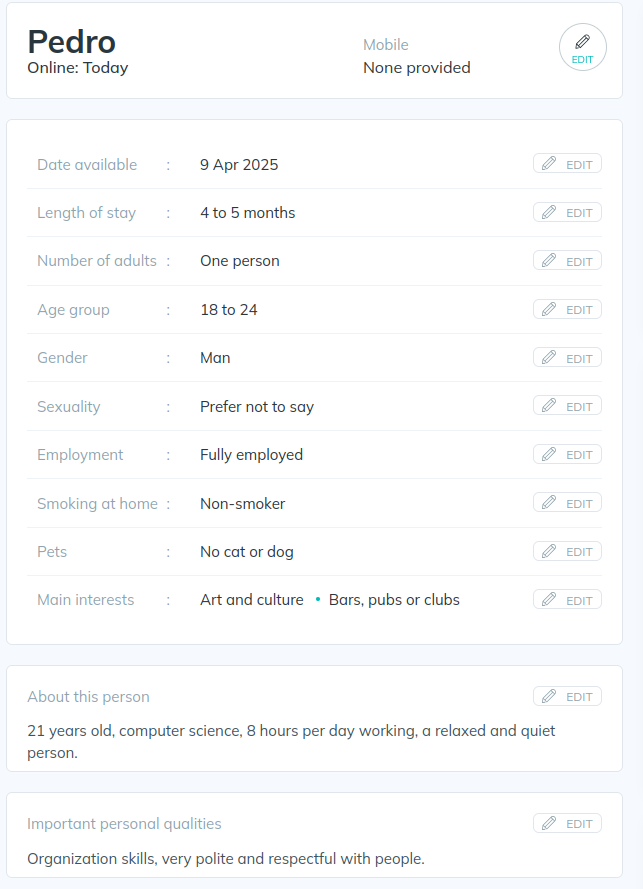
\includegraphics[width=0.8\textwidth]{fotos/perfil-flatmate.png}
    \caption{Configuración del perfil de usuario \textbf{}.}
\end{figure}
\begin{figure}[H]
    \centering
    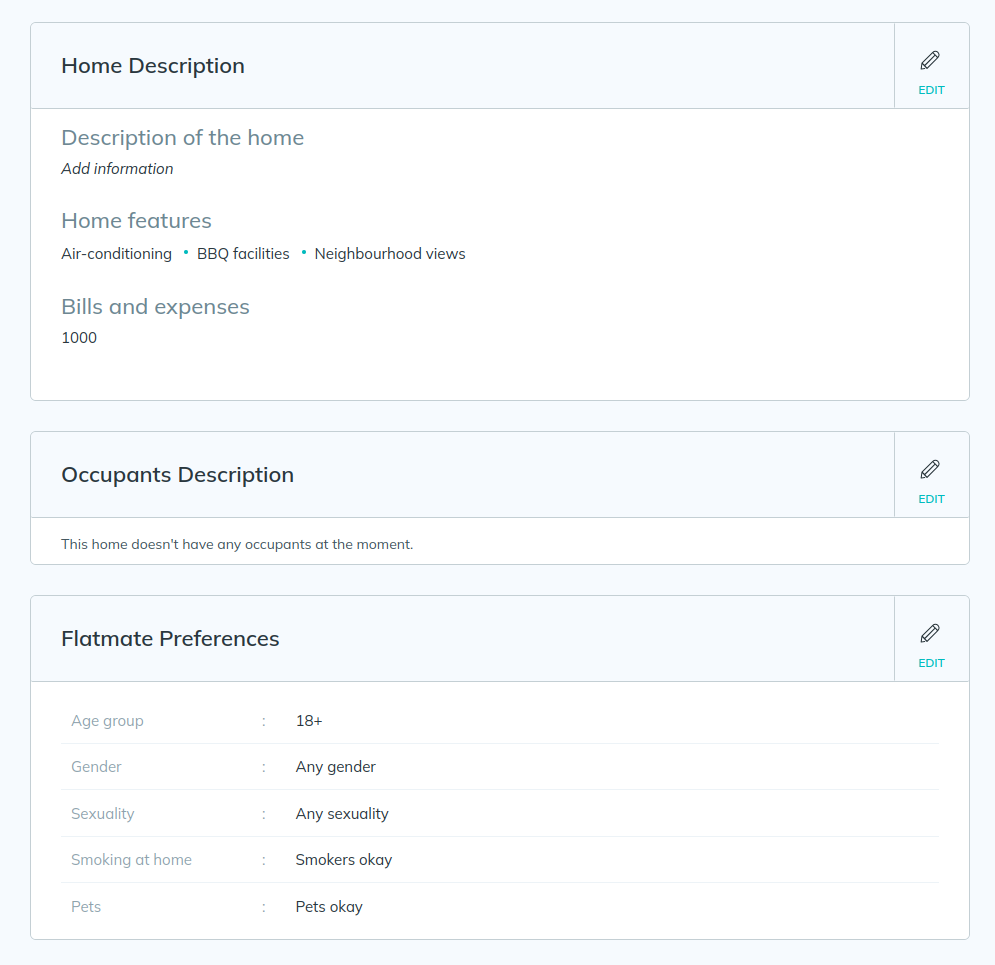
\includegraphics[width=0.8\textwidth]{fotos/home-flatmate.png}
    \caption{Configuración del perfil de la vivienda \textbf{}.}
\end{figure}
\subsubsection*{Interfaz y usabilidad}
La aplicación presenta una interfaz intuitiva con un buen tiempo de respuesta, la aplicación destaca por ser fácil de usar y ofrecer en todo momento información al usuario sobre las recomendaciones. Es de destacar que tanto la parte de ofertante como la de buscador tienen coherencia en cuanto a estilo y son muy personalizables.

\subsubsection*{Características destacadas}
\begin{itemize}
    \item  \textbf{Sistema de recomendación:} Utiliza un porcentaje de compatibilidad entre posible inquilino y vivienda, lo que facilita la búsqueda.
    \item \textbf{Explicación de compatibilidad:} Muestra un porcentaje indicando el grado de compatibilidad, además refleja las razones de incompatibilidad para dar "feedback" al usuario.
    \item \textbf{Configuración de perfil:} La creación de perfiles tanto para usuario como para propietario permite representar bien los intereses que se buscan en la comunidad o que tienen los usuario, siendo además sencillo y rápido de configurar. 
\end{itemize}
\begin{figure}[H]
    \centering
    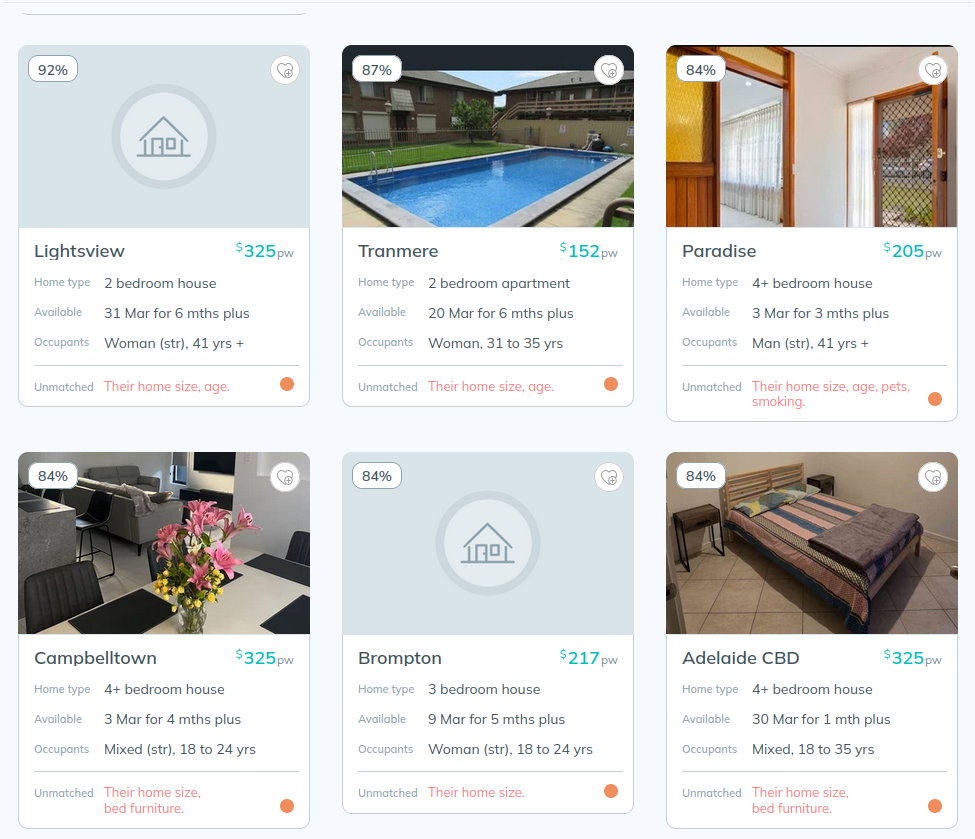
\includegraphics[width=1\textwidth]{fotos/flatmate-matches.png}
    \caption{Sección de búsqueda de vivienda por afinidad\textbf{}.}
\end{figure}
\subsubsection*{Limitaciones}
\begin{itemize}
    \item La aplicación únicamente está disponible en Australia, lo que limita enormemente su uso.
    \item No ofrece ningún tipo de herramienta para administrar las tareas de la vivienda una vez creado el piso compartido.
    \item La compatibilidad se basa en aspectos básicos como la edad, el género y si se es fumador, sin un análisis más profundo de la afinidad entre compañeros.
\end{itemize}

\subsubsection*{Conclusión}
Es una aplicación que ofrece una buena solución para buscar piso en función de afinidad, además el feedback que da al usuario con los porcentajes  e indicaciones sobre porque no coinciden son puntos muy favorables. Sin embargo, su única disponibilidad en Australia y la poca complejidad del algoritmo de recomendación provoca que no ofrezca una solución completa.

\subsection{Gestión de tareas en pisos compartidos}

\subsubsection{Flatify}
\emph{Flatify} \cite{Flatify} ofrece diversas funcionalidades enfocadas en la gestión de un piso compartido, entre las que destacan:
\begin{itemize}
    \item \textbf{Calendario compartido:} Permite añadir eventos para todos los integrantes.
    \item \textbf{Gestión de gastos:} Facilita el registro de pagos y el reparto de costes.
    \item \textbf{Lista de compras:} Los usuarios pueden añadir y marcar productos comprados.
    \item \textbf{Plan de limpieza:} Asigna tareas equitativamente entre los miembros del hogar.
    \item \textbf{Chat grupal:} Comunicación integrada para coordinarse fácilmente.
\end{itemize}

\begin{figure}[H]
    \centering
    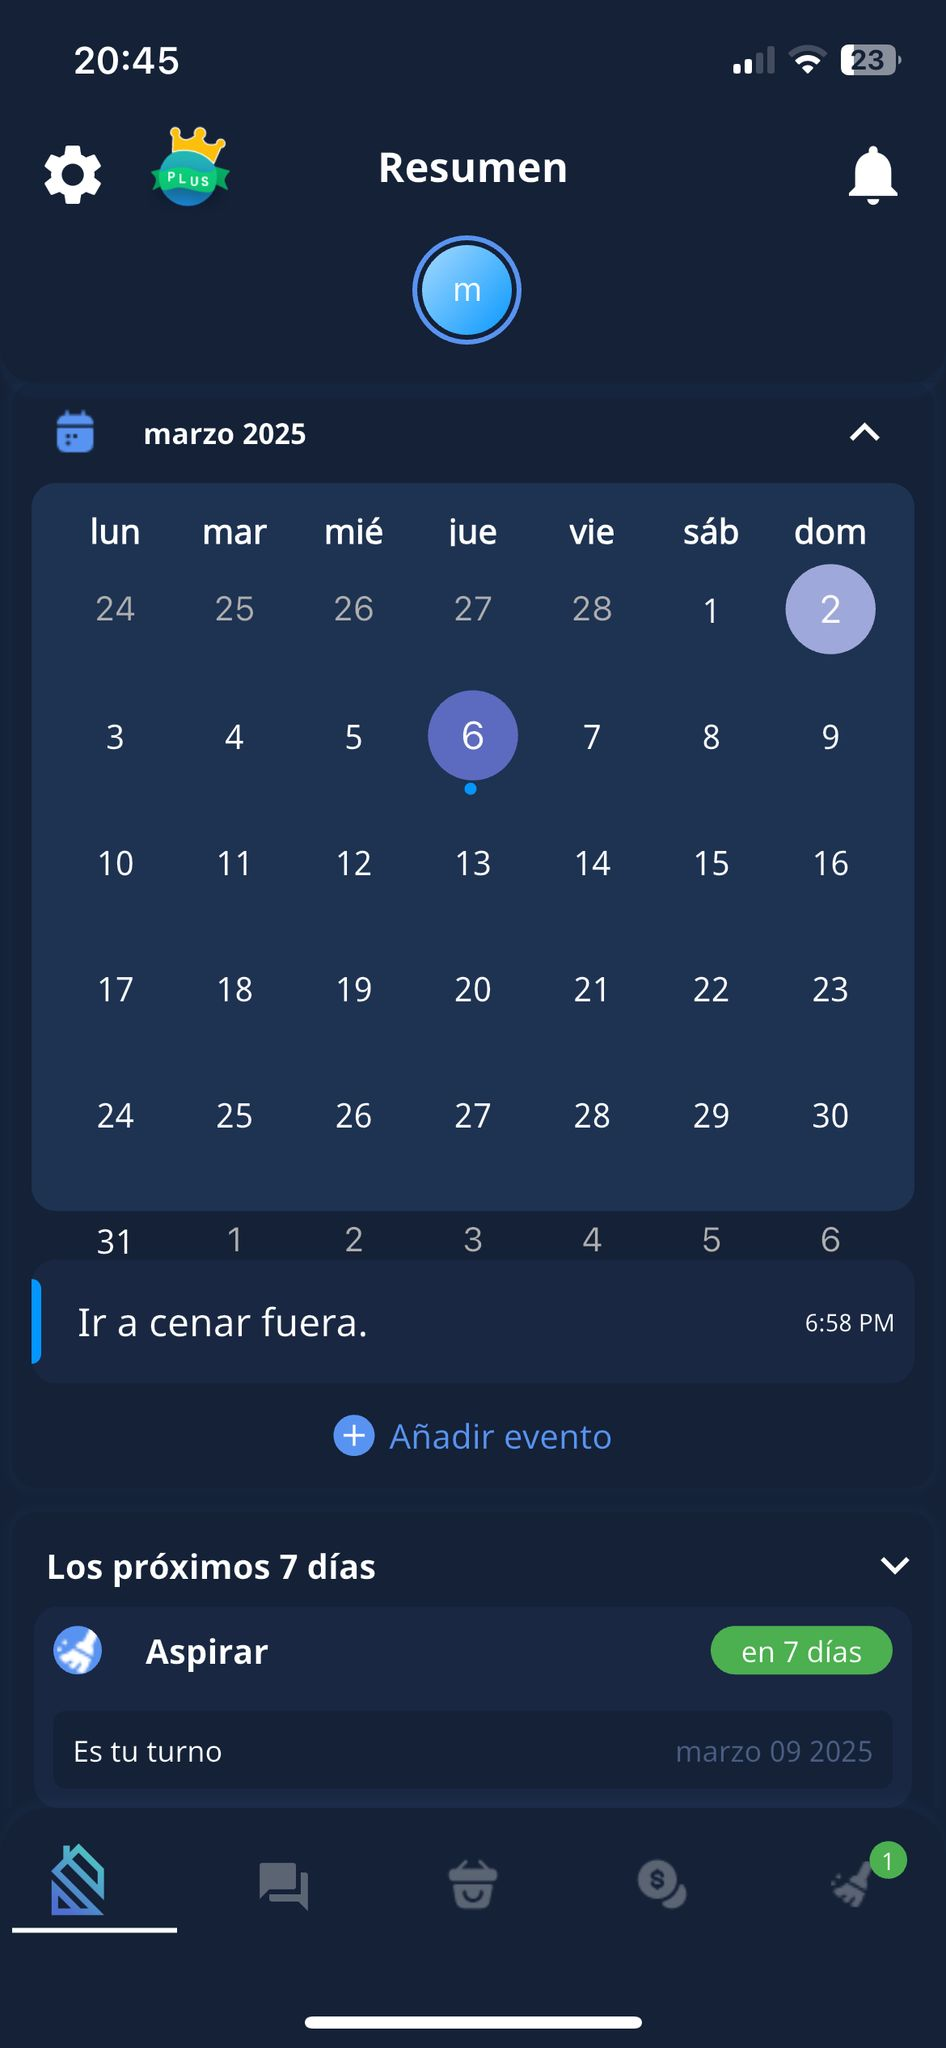
\includegraphics[width=0.4\textwidth]{fotos/Home-flatify.jpeg}
    \caption{Calendario de la aplicación\textbf{}.}
\end{figure}
\newpage
\subsubsection*{Interfaz y usabilidad}
La aplicación cuenta con una interfaz limpia e intuitiva, facilitando la navegación. Además, incluye una guía de primeros pasos útil para familiarizarse rápidamente con sus funciones.

\subsubsection*{Características destacadas}
\begin{itemize}
    \item \textbf{Distribución de tareas:} Permite establecer una secuencia de usuarios para rotar las responsabilidades de forma automática, asegurando una distribución justa.
    \item \textbf{Lista de compras:} Funciona correctamente, aunque la funcionalidad de subir facturas para gestionar los pagos está limitada a la versión premium.
    \item \textbf{Calendario:} Útil para eventos, pero no integra las tareas del hogar, lo que limita su funcionalidad.
\end{itemize}
\begin{figure}[H]
    \centering
    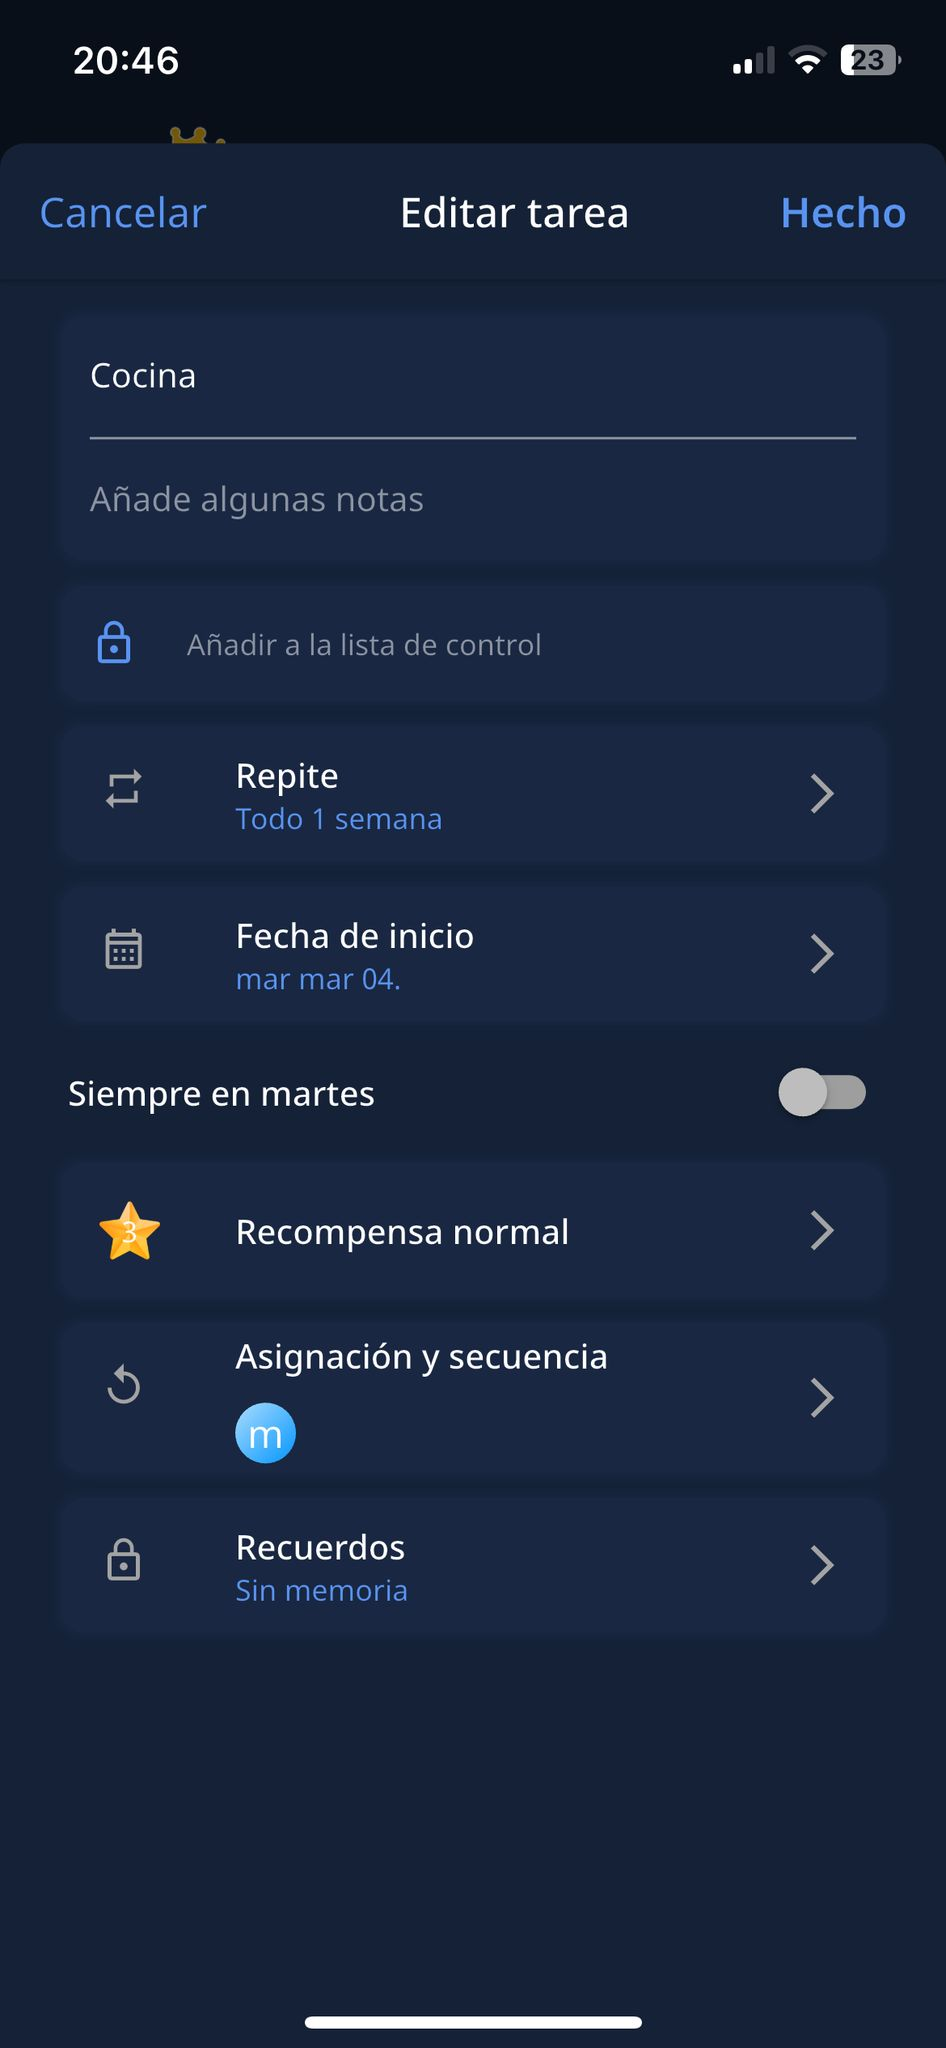
\includegraphics[width=0.4\textwidth]{fotos/creacion-tarea-flatify.jpeg}
    \caption{Sección para crear y editar una tarea\textbf{}.}
\end{figure}

\subsubsection*{Limitaciones}
\begin{itemize}
    \item Muchas características clave requieren pago o implican ver anuncios para su uso.
    \item La gestión de pagos y la lista de la compra no están bien sincronizadas, lo que reduce su utilidad.
    \item El calendario no permite gestionar tareas, desaprovechando su potencial.
\end{itemize}
\subsubsection*{Conclusión}
A pesar de las limitaciones de su versión gratuita, esta aplicación es la mejor solución encontrada para la gestión de pisos compartidos, ya que ofrece diversas herramientas útiles para la organización del hogar. Sin embargo, presenta algunos inconvenientes como una funcionalidad de calendario que resulta incompleta y la ausencia de herramientas para la creación de hogares basados en afinidades. Estas carencias hacen que la aplicación no sea una opción viable para nuestro problema.

\section{Tecnologías en el mercado}
Para el desarrollo del sistema será necesario apoyarse en diferentes tecnologías que permitan constuir un sistema que responda a las necesidades planteadas.
Con el actual auge del desarrollo software, numerosas tecnologías están apareciendo en el mercado para facilitar y mejorar la calidad del desarrollo. A continuación, se realiza un análisis de las tecnologías más relevantes y las ventajas que pueden ofrecer.

\begin{figure}[H]
    \centering
    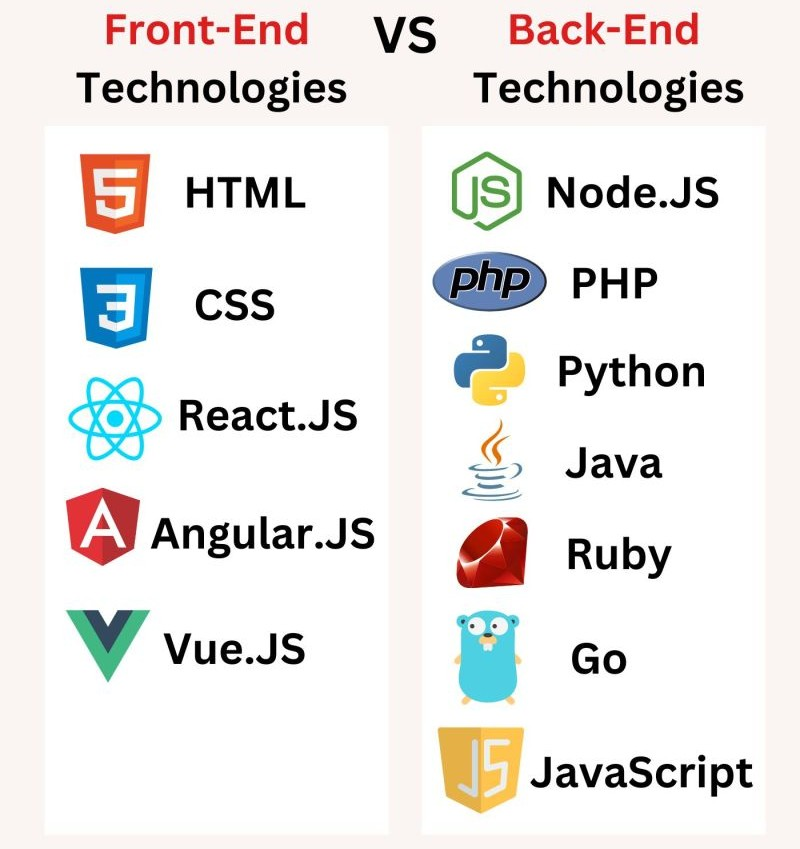
\includegraphics[width=0.45\textwidth]{fotos/lenguajes.jpg}
    \caption{Lenguajes de programación y tecnologías presentes en el mercado\textbf{}.}
    \label{fig:lenguajes-programacion}
\end{figure}
\subsection{Back-End}
\subsubsection*{Python-Django}
Con el aumento de popularidad de Python \cite{Top_Language_GitHub}, varios frameworks han aparecido para llevar su funcionamiento al Back-End, como se muestra en la imagen \ref{fig:lenguajes-programacion}. Entre ellos, destacan FastAPI, Django y Flask. Estos frameworks aprovechan las ventajas de Python, un lenguaje orientado a la legibilidad y popularizado por el auge de la inteligencia artificial. Django es el más destacable por su robustez y numerosas utilidades. Aunque FastAPI y Flask son excelentes para desarrollar APIs por ser ligeros y especializados, siendo más adecuados para aplicaciones menores, mientras que Django cubre aplicaciones complejas que requieren escalabilidad o seguridad a partir del uso del patrón MVC \cite{MVC}.

\subsubsection*{NodeJS- Express}
NodeJS\cite{NodeJS} ha revolucionado el desarrollo Back-End al permitir la ejecución de código JavaScript en el lado del servidor, facilitando así la unificación de tecnologías utilizadas tanto en el Front-End como en el Back-End, como muestra la imagen \ref{fig:lenguajes-programacion}, con tecnologías como React en el Front-End y NodeJS en el Back-End. Entre sus características principales se encuentra su gestión de la asincronía mediante un modelo no bloqueante que utiliza un ``event loop``, lo cual permite procesar solicitudes sin bloquear el hilo principal, tal como se muestra en la Figura \ref{fig:nodejs}. Además, ofrece facilidad para trabajar con objetos JavaScript similares a JSON y ha dado lugar a la aparición de frameworks que lo complementan; en este caso, nos centraremos en Express, que facilita la gestión de rutas y la creación de aplicaciones web escalables.
\begin{figure}[H]
    \centering
    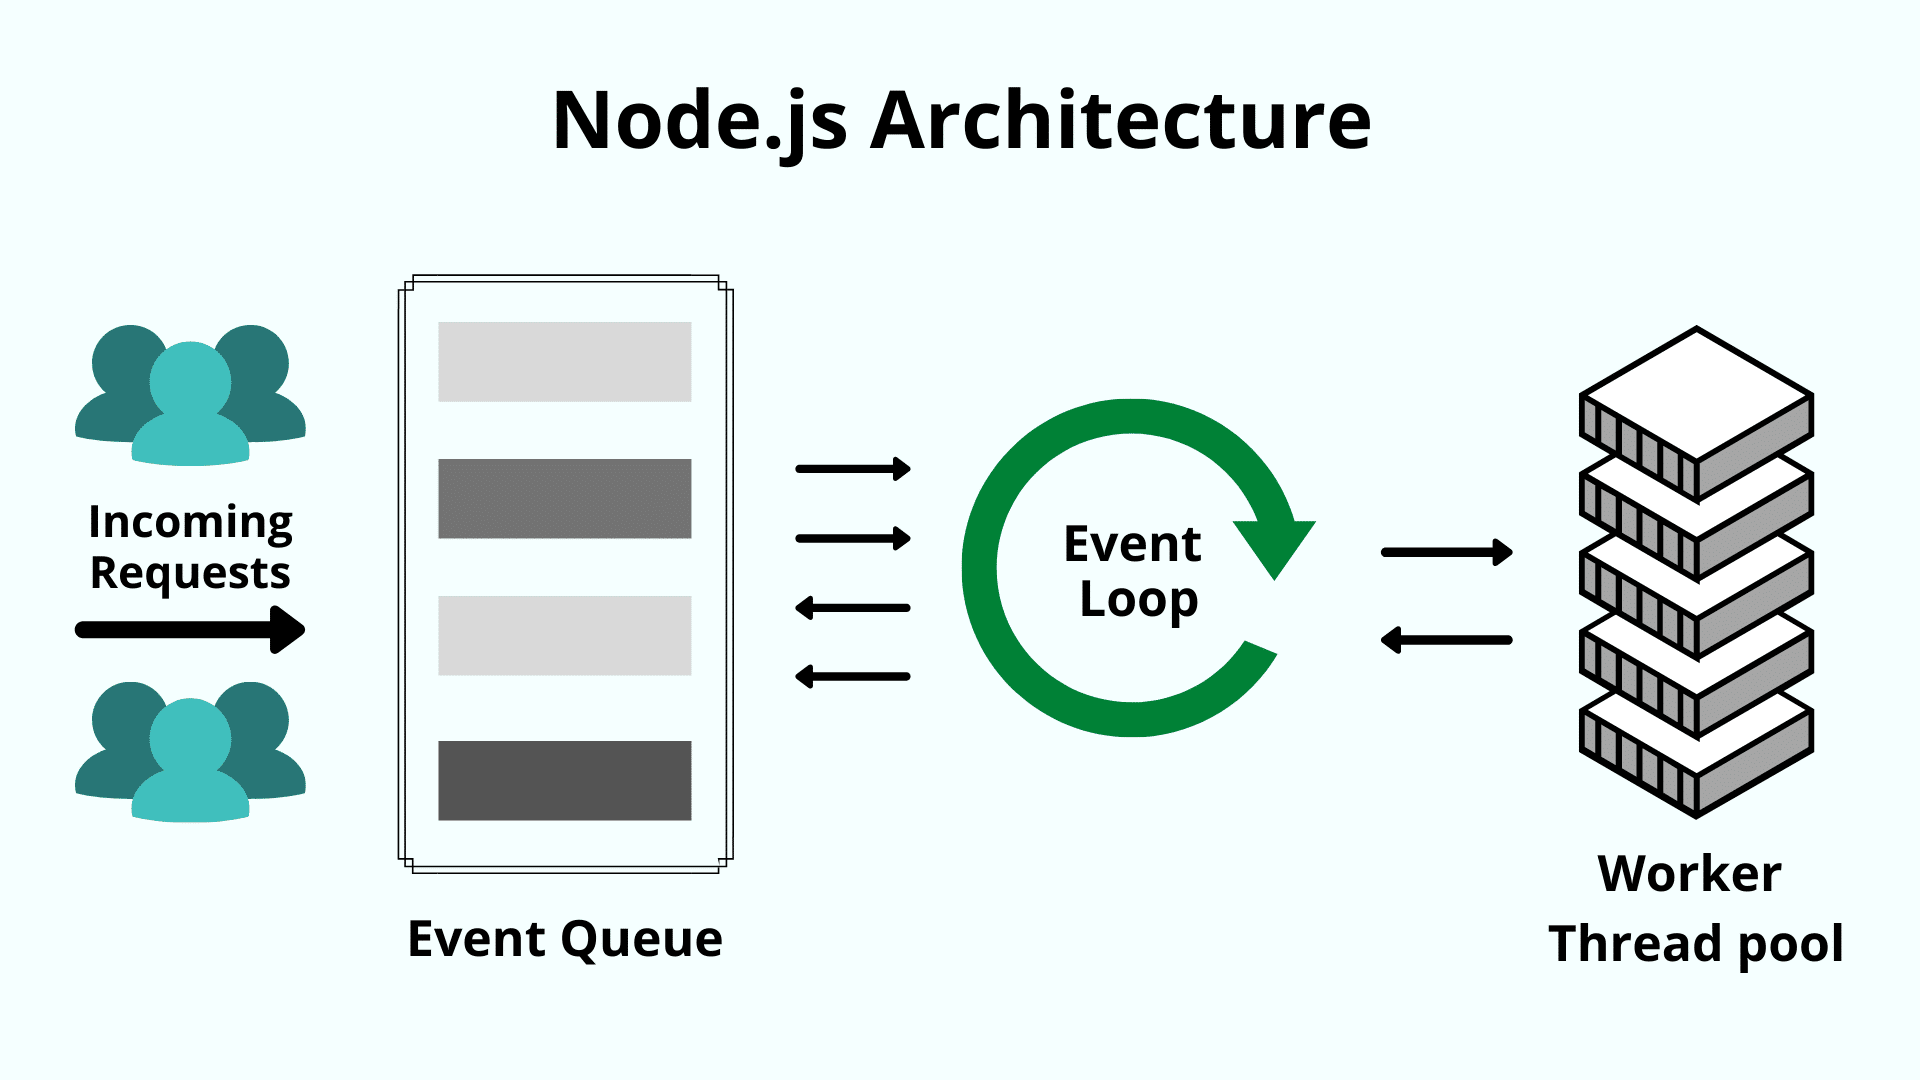
\includegraphics[width=1\textwidth]{fotos/node-js2.png}
    \caption{Arquitectura NodeJS\textbf{}.}
    \label{fig:nodejs}
\end{figure}
\subsubsection*{Java}
Java, conocido por su fuerte tipado y su compilación, ofrece una solución robusta para el desarrollo Back-End con Spring Boot. Este framework simplifica la gestión de dependencias, proporcionando una estructura más fácil de manejar que la versión anterior de Spring. Es ampliamente utilizado en entornos empresariales debido a su capacidad para soportar arquitecturas complejas, como microservicios o arquitectura hexagonal. Además, Spring Boot promueve prácticas avanzadas de desarrollo como la inyección de dependencias y sus starters, los cuales se pueden apreciar en la imagen \ref{fig:spring}, incluyen desde seguridad hasta manejo reactivo de peticiones. Es una opción robusta para aplicaciones a gran escala. 
\begin{figure}[H]
    \centering
    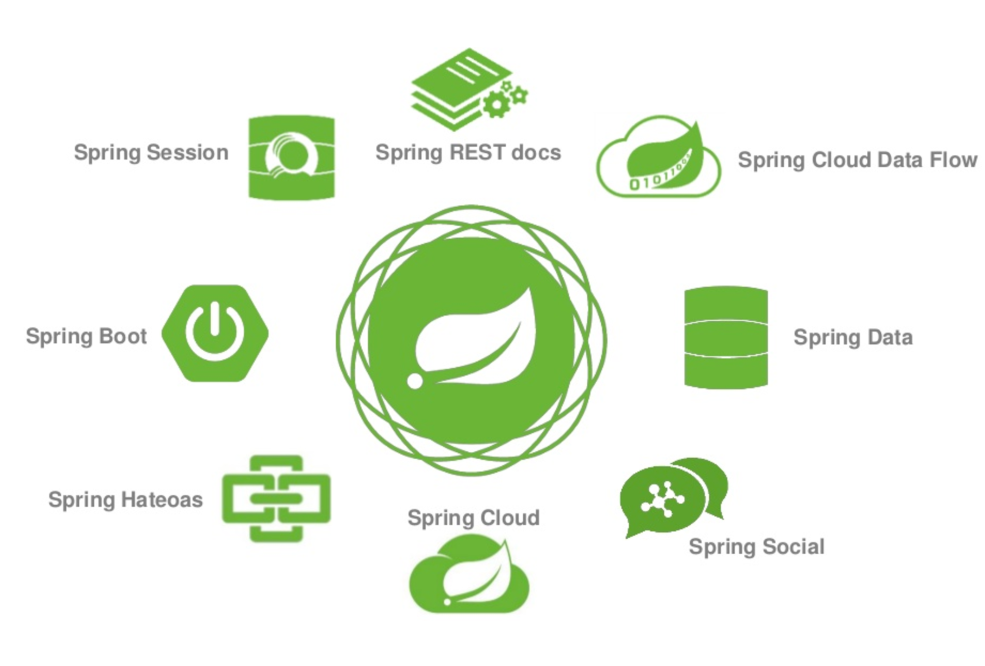
\includegraphics[width=0.8\textwidth]{fotos/tete.png}
    \caption{Starters de Spring Boot\textbf{}.}
    \label{fig:spring}
\end{figure}
\subsection{Front-End}
En el desarrollo Front-End, JavaScript se ha consolidado como el estándar principilar con la aparición de numerosos frameworks. A continuación se van a analizar las opciones más interesantes para la parte visual de la aplicación.
\subsubsection*{React}
React es en la actualidad la biblioteca de desarrollo Front-End más demandada \cite{Frontend_Frameworks_DevJobsScanner}. Su enfoque basado en la creación de componentes reutilizables, el uso de JSX que permite escribir código similar a HTML dentro de archivos JavaScript, como se puede observar en la imagen \ref{fig:react}, junto con la gestión de estados y hooks,  permite estructurar aplicaciones de manera escalable y eficiente de forma sencilla. Además su amplica adopción y su extensa comunidad y documentación lo convierten en una gran herramienta a la hora de crear interfaces complejas y dinámicas.
\begin{figure}[H]
    \centering
    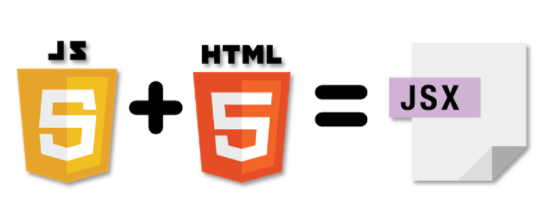
\includegraphics[width=0.8\textwidth]{fotos/react.PNG}
    \caption{Explicación del concepto JSX\textbf{}.}
    \label{fig:react}
\end{figure}
\subsubsection*{Angular}
Angular es un framework más completo y estructurado en comparación con React, que se centra más en ofrecer al usuario herramientas listas para usar. Sigue también el concepto de componentes pero con un enfoque más estricto en cuanto a arquitectura y estructura del proyecto, lo cual ayuda en la creación de aplicaciones robustas y mantenibles.

\subsubsection*{TypeScript}
El notable crecimiento en la popularidad de TypeScript se debe a que proporciona un sistema de tipado estático sobre JavaScript, lo cual ayuda a reducir errores en tiempo de compilación y mejora la detección de errores y legibilidad del código como se muestra en la imagen \ref{fig:ts}. TypeScript se está convirtiendo en un estándar dentro del desarrollo Front-End profesional debido a la gran ayuda que ofrece para detectar de forma temprana errores y su integración con cualquier tipo de framework moderno como React y Angular.
\begin{figure}[H]
    \centering
    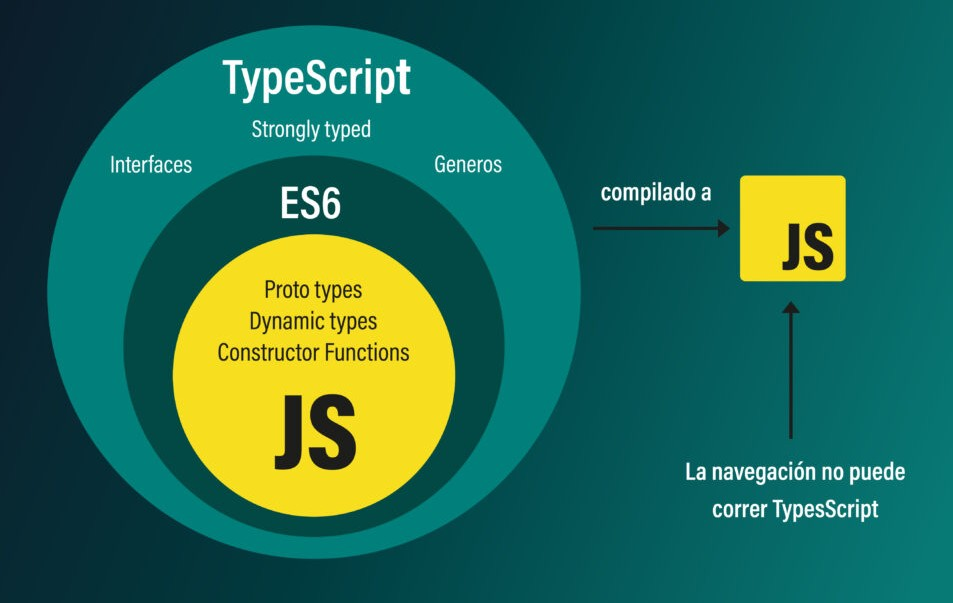
\includegraphics[width=0.8\textwidth]{fotos/typescript.jpg}
    \caption{Explicación del concepto de TypeScript\textbf{}.}
    \label{fig:ts}
\end{figure}

\subsection{Base de Datos}
\begin{figure}[H]
    \centering
    
\includegraphics[width=0.3\textwidth]{fotos/postgre.png}
    \caption{Logo PostgreSQL\textbf{}.}
    \label{fig:psql}
\end{figure}
\subsubsection*{PostgreSQL}
PostgreSQL \ref{fig:psql} es una base de datos relacional \textit{open source} que se destaca por su alto rendimiento, escalabilidad y fiabilidad. Garantiza transacciones \textit{ACID} (Atomicidad, Consistencia, Aislamiento y Durabilidad) \cite{cics-acid}, lo que asegura que las operaciones en la base de datos se realicen de forma segura y consistente. Además, PostgreSQL ofrece una robusta seguridad y es respaldada por una comunidad activa que mantiene una documentación extensa y detallada.
\begin{figure}[H]
    \centering
    
\includegraphics[width=0.5\textwidth]{fotos/mongo.png}
    \caption{Logo MongoDB\textbf{}.}
    \label{fig:mongo}
\end{figure}
\subsubsection*{MongoDB}
MongoDB \ref{fig:mongo} es una base de datos no relacional que almacena los datos en formato BSON (Binary JSON), lo que le permite manejar grandes volúmenes de datos de manera eficiente. Se caracteriza por su alto rendimiento, flexibilidad y facilidad para integrarse con aplicaciones modernas. A diferencia de las bases de datos relacionales, MongoDB no requiere esquemas estrictos, lo que lo hace ideal para manejar datos no estructurados o semi-estructurados, facilitando la evolución y adaptación de los modelos de datos.

\section{Conclusión tras estudiar el mercado}
Tras analizar diversas alternativas disponibles en el mercado, hemos identificado aplicaciones que abordan parcialmente la problemática planteada. \textit{Flatmate Finders} facilita la búsqueda de compañeros de piso en función de la afinidad, mientras que \textit{Flatify} destaca en la gestión de la convivencia, ofreciendo herramientas para la organización de tareas, calendario compartido y lista de la compra.

Sin embargo, ninguna de estas soluciones integra ambas funcionalidades en una única plataforma. La falta de una aplicación que combine tanto la búsqueda de vivienda como su gestión diaria con todos los requisitos necesarios, evidencia la necesidad de desarrollar este proyecto, ofreciendo una solución integral que cubra todas las necesidades de la vida en pisos compartidos basado en el \emph{co-housing}. En cuanto a las tecnologías todas las comentadas cumplen con los requisitos mínimos de funcionalidad para poder llevar a cabo el proyecto, por tanto la tecnología escogida dependerá de la arquitectura, preferencia del equipo de desarrollo y complejidad de la aplicación.

    \chapter{Especificación de Requisitos} \label{requisitos}

\section{Propósito}
En este capítulo se definirán las distintas características, funcionalidades y restricciones que debe cumplir la aplicación que se va a desarrollar. Se redactará un conjunto de requisitos esenciales que guiarán el proceso de creación del sistema. Además, se describirán los requisitos de las interfaces visuales, estableciendo un patrón a seguir durante el desarrollo de la aplicación.

\section{Alcance}
El sistema tiene como objetivo proporcionar a los usuarios una solución eficaz para la búsqueda y gestión de viviendas compartidas, alineada con los principios del \textit{co-housing}. Este proyecto abordará las siguientes tareas principales:

\begin{itemize}
    \item Registro y gestión de usuarios.
    \item Registro y gestión de comunidades.
    \item Recomendación de viviendas por afinidad.
    \item Gestión de tareas y actividades.
\end{itemize}

Los datos serán almacenados en bases de datos, y se hará especial énfasis en la escalabilidad y robustez de la aplicación, con el objetivo de garantizar un rendimiento escalable y efectivo.


\section{Definiciones, siglas y abreviaturas}
\begin{itemize}
    \item \textbf{Usuario Buscador:} Persona que se da de alta en la plataforma con el rol de \textit{Buscador}. Su objetivo es buscar comunidades y unirse a ellas. Puede enviar solicitudes e interactuar con el gestor de tareas.
    \item \textbf{Usuario Ofertante:} Persona que registra una comunidad en la plataforma, introduciendo datos específicos como fotos, metros cuadrados, número de habitaciones, entre otros. Se le ofrecerá funcionalidad para administrar la comunidad, definiendo sus criterios de afinidad y gestionando las solicitudes de unión, aceptándolas o rechazándolas.
    \item \textbf{Comunidad:} Concepto que hace referencia a la vivienda compartida entre varios integrantes. Esta podrá ser gestionada a través de actividades y tareas que se propondrán y deberán ser realizadas por los integrantes de la comunidad.
    \item \textbf{ShareSpace:} Nombre por el que será identificado el proyecto, por tanto a partir de ahora su uso referencia a la aplicación.
\end{itemize}



\section{Perspectiva del producto}
Este sistema tiene como objetivo ofrecer una solución eficiente que adapte las distintas necesidades de los usuarios.
A medida que la aplicación vaya creciendo se podría integrar nueva funcionalidad que aporte valor añadido a la experiencia del usuario.
De forma inicial la aplicación se construirá en torno a distintos servicios que encapsularán parte de la lógica de negocio. Como se puede ver en la imagen \ref{fig:diagrama-componentes} estos componentes se comunicarán con la interfaz gráfica, facilitando la experiencia de usuario de manera sencilla y accesible.
\newpage
\begin{figure}[H]
    \centering
    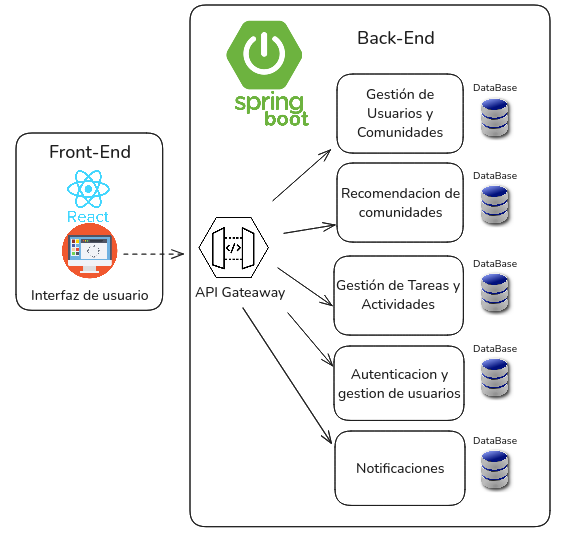
\includegraphics[width=0.8\textwidth]{fotos/diagrama-componentes.png}
    \caption{Diagrama interacción entre componentes\textbf{}.}
    \label{fig:diagrama-componentes}
\end{figure}
\section{Restricciones}
Las restricciones principales de la aplicación para que la experiencia sea la adecuada tanto en móvil como en ordenador serán las siguientes:

\begin{itemize}

    \item \textbf{Hardware:}
    \begin{itemize}
        \item Se recomienda tener al menos 8 GB de RAM para un rendimiento óptimo cuando se usen múltiples pestañas o aplicaciones al mismo tiempo.
    \end{itemize}

   \item \textbf{Navegadores Web:}
    \begin{itemize}
        \item Google Chrome versión 90 o superior.
        \item Mozilla Firefox versión 80 o superior.
        \item Safari 14.0 o superior.
        \item Microsoft Edge versión 90 o superior.
    \end{itemize}
    \item \textbf{Sistemas Operativos Compatibles:}
    \begin{itemize}
        \item \textbf{Windows:} Windows 10 o superior.
        \item \textbf{macOS:} macOS 10.15 o superior.
        \item \textbf{Linux:} Cualquier distribución moderna de Linux, como Ubuntu 20.04 o superior.
    \end{itemize}
\end{itemize}
\section{Funciones del producto}
El sistema contará con una serie de funcionalidades clave para garantizar su cumplimiento del objetivo establecido. A continuación, se detallan las principales funciones que ofrecerá la plataforma:
\begin{itemize}
    \item \textbf{Registro de usuarios y comunidades:} El sistema permitirá registrar tanto a usuarios como a comunidades, gestionando sus respectivos datos. Los usuarios podrán crear su perfil y las comunidades podrán ser configuradas con detalles como ubicación, número de habitaciones, y características específicas.
    \item \textbf{Búsqueda de comunidad:} La plataforma ofrecerá recomendaciones de comunidades basadas en afinidad y preferencias del usuario. Además, permitirá enviar solicitudes de unión a los propietarios de las comunidades, estableciendo una comunicación directa entre ambos para facilitar el proceso de integración.
    \item \textbf{Gestión de tareas:} Los usuarios podrán registrar nuevas tareas, asignarlas a la  comunidad y consultar el estado de las que tienen que realizar. Las tareas estarán integradas en un calendario compartido, asegurando que todos los miembros estén al tanto de las actividades pendientes y los plazos de realización.
    \item \textbf{Gestión de eventos y actividades:} Se podrán crear y gestionar eventos dentro de la comunidad, desde reuniones hasta actividades sociales, fomentando la convivencia.
\end{itemize}

\section{Redacción de requisitos}
Los requisitos van a describir de forma clara y directa las características que el sistema debe proporcionar.  
Vamos a encontrar tres secciones generales:

\begin{itemize}
    \item \textbf{Requisitos funcionales:} Definen las funciones que la aplicación debe ser capaz de realizar.
    \item \textbf{Requisitos no funcionales:} Evaluaran cómo debe comportarse el sistema, dentro de ellos se definiran los requisitos de seguridad.
    \item \textbf{Requisitos de interfaces:} Especificarán los criterios a seguir en el apartado visual, el análisis de las interfaces de usuarios se va a realizar a partir de dos bocetos.
\end{itemize}

Los requisitos funcionales se agruparán en función de grandes bloques de funcionalidad.

\section{Requisitos funcionales}

\subsection{Bloque Gestión de Usuarios y Autenticación}

\begin{itemize}
    \item \textbf{RF-01: Registro de Usuarios}  
    Los usuarios podrán registrarse como buscadores u ofertantes en la aplicación mediante un formulario que recopile información básica. Los campos mínimos requeridos son:
    \begin{itemize}
        \item Nombre
        \item Correo Electrónico
        \item Contraseña
        \item Localización
        \item Afinidad
    \end{itemize}
    
    \item \textbf{RF-02: Inicio de Sesión}  
    Los usuarios podrán iniciar sesión introduciendo su correo electrónico y contraseña previamente registrados.  
    En caso de error en los datos, el sistema notificará al usuario con un mensaje adecuado.
    
    \item \textbf{RF-03: Gestión de Perfiles}  
    Los usuarios deberán poder visualizar y modificar sus datos personales, como la localización y preferencias de afinidad.

    \item \textbf{RF-04: Eliminación de Usuario}
    Los usuarios podrán borrar su cuenta del sistema, eliminando toda información asociada con ellos.
\end{itemize}

\subsection{Bloque Gestión de Comunidades}

\begin{itemize}
    \item \textbf{RF-05: Creación de Comunidades}  
    Los ofertantes podrán crear nuevas comunidad mediante un formulario que incluirá:
    \begin{itemize}
        \item Imágenes representativas
        \item Descripción detallada de la comunidad
        \item Criterios de afinidad para los miembros
        \item Número de integrantes deseado
    \end{itemize}
    
    \item \textbf{RF-06: Unión a Comunidades}  
    Los propietarios deben recibir una notificación cuando un usuario solicite unirse a una comunidad pudiendo ver su información y aceptarlo o rechazarlo.

    \item \textbf{RF-07: Petición de Unión}  
    Los usuarios podrán solicitar unirse a una comunidad concreta mediante un proceso de petición sencilla.

    \item \textbf{RF-08: Notificación de respuesta a Unión}  
    Los usuarios serán notificados con la decisión del propietario de la comunidad a la que han pedido unirse.

    \item \textbf{RF-09: Eliminación de Comunidad}  
    Los propietarios deben poder eliminar la comunidad que han registrado previamente, eliminando toda la información contenida en el sistema.

    \item \textbf{RF-10: Gestión de Comunidad}  
    Los usuarios ofertantes podrán modificar los datos del perfil de la comunidad.


    
\end{itemize}

\subsection{Bloque Gestión de Tareas}

\begin{itemize}
    \item \textbf{RF-11: Creación de Tareas/Eventos}  
    Los usuarios podrán crear tareas/eventos comunitarios mediante un formulario sencillo donde introducirán mínimo: el nombre, una descripción breve y la frecuencia con la que se deberá realizar.
    
    \item \textbf{RF-12: Gestión del Calendario}  
    El sistema debe mostrar un calendario personalizado a cada usuario, que incluirá:
    \begin{itemize}
        \item Tareas asignadas
        \item Eventos destacados
    \end{itemize}
    
    \item \textbf{RF-13: Visibilidad de las Tareas}  
    Los usuarios podrán ver la descripción detallada de cada tarea que se les haya asignado, incluyendo fechas de realización y compañeros con los que tienen que colaborar.
    
    \item \textbf{RF-14: Marcar Tareas}  
    Los usuarios deberán poder marcar las tareas como completadas y consultar el estado de las tareas pendientes con su respectiva fecha límite.

    \item \textbf{RF-15: Reparto de Tareas}  
    El sistema distribuirá las tareas semanalmente de manera justa, asignando responsabilidades en un orden secuencial.

    \item \textbf{RF-16: Flexibilidad en la Asignación de Tareas}  
    Los usuarios podrán distribuir de forma libre sus tareas asignadas a lo largo de la semana.
\end{itemize}

\subsection{Bloque Recomendación de Comunidades}

\begin{itemize}
    \item \textbf{RF-17: Recomendación de Comunidades}  
    El sistema recomendará comunidades que coincidan con los criterios tanto de afinidad como de vivienda introducidos por los usuarios.
    
    \item \textbf{RF-18: Guardar Comunidades de Interés}  
    El usuario podrá guardar sus comunidades de interés utilizando un botón de “guardar” o “me gusta”.
    
    \item \textbf{RF-19: Grado de afinidad}  
    El sistema mostrará a los usuarios el grado de afinidad que existe entre una comunidad y ellos con un porcentaje sobre cien.
\end{itemize}

\section{Requisitos No Funcionales}
\begin{itemize}
    \item \textbf{RNF-01: Notificaciones}  
    Las notificaciones deben ser rápidas y entregarse a los usuarios en un período de tiempo corto (entorno a uno o dos segundos).
    
    \item \textbf{RNF-02: Mantenibilidad y Escalabilidad}  
    El sistema debe estar diseñado para ser fácil de mantener, pudiendo escalar a medida que crecen los usuarios y las funcionalidades.
    
    \item \textbf{RNF-03: Alta Disponibilidad}  
    El sistema debe permanecer operativo en todo momento, asegurando que si aparece un fallo en alguna parte del sistema el resto de servicios seguirán operativos.
    
    \item \textbf{RNF-04: Soporte de Carga}  
    El sistema debe soportar un volumen de usuarios considerable de forma simultánea, asegurando que el servicio esté disponible ante un flujo alto de usuarios.

    \item \textbf{RNF-05: Mantenimiento}
    El sistema debe permitir al administrador realizar tareas de mantenimiento sin afectar el servicio a los usuarios
    \item \textbf{RFN-06: Gestión de Usuarios}
    El sistema debe poder permitir al administrador gestionar los usuarios pudiendo activar/desactivar cuentas y modificar roles.
    \item \textbf{RFN-07: Monitoreo}
    El sistema debe alertar al usuario en caso de caídas de servicio que afecten a los usuarios.
\end{itemize}

\subsection{Requisitos de Seguridad}
\begin{itemize}
    \item \textbf{RNF-08: Autorización y autenticación}  
     La aplicación deberá contar con un sistema de autenticación y autorización seguro que garantice el control de los accesos.
    
    \item \textbf{RNF-09: Seguridad en Base de Datos}  
    El sistema debe implementar mecanismos de seguridad que protegan a las bases de datos de accesos no autorizados.
    
    \item \textbf{RNF-10: Protección contra Inyecciones SQL}  
    El sistema debe prevenir ataques de inyección SQL mediante el uso de validaciones adecuadas en los datos de entrada.
    \item \textbf{RNF-11: Protección de datos}
    El sistema debe asegurar el cumplimiento de las normativas vigentes de  \href{https://eur-lex.europa.eu/ES/legal-content/summary/general-data-protection-regulation-gdpr.html}{protección de datos de la Unión Europea}, para garantizar un uso adecuado de los datos personales.
\end{itemize}

\subsection{Requisitos de Interfaces Externas}
Dentro de las interfaces externas distinguimos dos grandes bloques, las APIs y las Interfaces de usuario:

\subsubsection{APIs}
Cada servicio del sistema expondrá sus operaciones a través de una API, lo que permitirá una comunicación eficiente entre los módulos.


\subsubsection{Interfaces de Usuario}

La interfaz de usuario permitirá un uso de la funcionalidad ofrecida por el sistema claro y sencillo.

Cada interfaz va a cumplir una serie de criterios de usabilidad y una estética uniforme. A modo de ejemplo se va a presentar dos bocetos esquematizados para presentar el flujo de diseño a seguir.

\subsubsection*{Página de Bienvenida}
La ''Landing Page'' tiene como objetivo ser la puerta de entrada a la aplicación para el usuario, por lo tanto tiene que ser directa y llamativa para captar su atención.
\newpage
\begin{figure}[H]
    \centering
    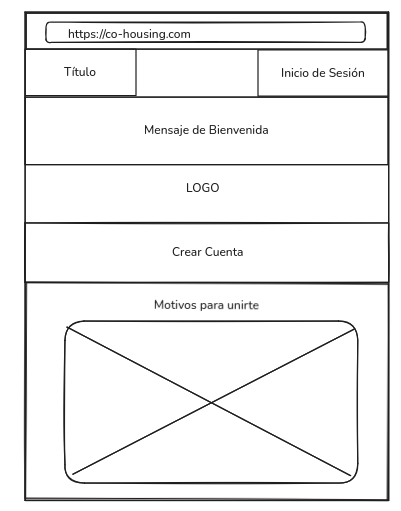
\includegraphics[width=0.8\textwidth]{fotos/home-basico.png}
    \caption{Boceto ''Landing Page''\textbf{}.}
    \label{fig:landing-page}
\end{figure}
\subsubsection*{Descripción:}
La imagen \ref{fig:landing-page} muestra la página a la que accede el usuario mediante el buscador al introducir el nombre de la aplicación, esta tiene como objetivo mostrar una pequeña presentación de la app y permitir la realización de una acción muy concreta, en este caso registrarse o iniciar sesión.

\newpage

\subsubsection*{Página Buscador}
La página del buscador tiene como objetivo poner en contacto a los usuarios con comunidades afines por lo que se debe mostrar la información de manera clara y bien estructurada.

\begin{figure}[H]
    \centering
    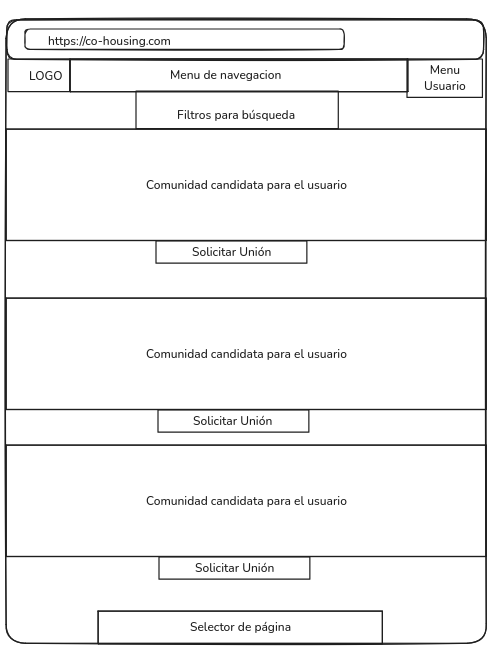
\includegraphics[width=0.8\textwidth]{fotos/buscador-basico.png}
    \caption{Boceto Página Buscador\textbf{}.}
    \label{fig:buscador-page}
\end{figure}
\subsubsection*{Descripción}
La imagen \ref{fig:buscador-page}  muestra la página que visualizará el usuario cuando accede a la sección ''Buscador'' de la aplicación,en ella aparecen las distintas comunidades sugeridas y un botón para solicitar la unión, además cuenta con un menú de navegación y un menú para el usuario.



    \input{secciones/05_Planificación}
    \input{secciones/06_Análisis}
    \input{secciones/07_Diseño}
    \chapter{Implementación} \label{diseño}

A continuación se procederá a explicar la implementación de las funcionalidades más representativas dentro del sistema, explicando su lógica, flujo y estructura. Además, se hará una presentación de las herramientas que han complementado el desarrollo de la aplicación de forma profesional y eficiente.

\section{Herramientas}

Durante todo el ciclo de vida del proyecto se han utilizado diversas herramientas que han complementado las distintas fases del desarrollo, desde la construcción de código hasta la integración continua (CI/CD), control de versiones y contenedorización.

\subsection{VSCode IDE}
\begin{figure}[H]
  \centering
  
\includegraphics[width=0.2\textwidth]{fotos/vs.png}
  \caption{Logo IDE VSCode}
\end{figure}
Como entorno de desarrollo integrado (IDE) se ha utilizado Visual Studio Code (VSCode), un editor de código fuente desarrollado por Microsoft \cite{vscode}. VSCode ha sido escogido por el gran número de extensiones gratuitas que ofrece, permitiendo trabajar con múltiples tecnologías y lenguajes de programación simultáneamente. Su integración con sistemas de control de versiones(GitHub) y herramientas de desarrollo lo convierte en una gran opción para proyectos software profesionales.

\subsection{GitHub}
\begin{figure}[H]
  \centering
  
\includegraphics[width=0.3\textwidth]{fotos/git.png}
  \caption{Logo GitHub}
\end{figure}
GitHub ha desempeñado un papel central durante el desarrollo del proyecto, no solo como plataforma de control de versiones, sino también como una herramienta clave para la automatización del desarrollo mediante GitHub Actions \cite{GithubActions} y su sistema de integración y entrega continua (CI/CD). Gracias a estas funcionalidades, ha sido posible estructurar y automatizar el ciclo de vida del desarrollo de forma organizada y eficiente.

El repositorio del proyecto está disponible en: 
\href{https://github.com/alonsodm12/TFG_COHOUSING}{Repositorio en GitHub}


\subsubsection*{Flujo de desarrollo}

El repositorio asociado al proyecto cuenta con tres ramas principales permitiendo una gestión organizada del desarrollo:

\begin{itemize}
    \item \textbf{main}: Rama asociada al entorno de producción, en ella se integran las iteraciones finalizadas que representan versiones estables y listas para ser desplegadas.
    \item \textbf{develop}: Rama de desarrollo, en ella se integran las tareas y las historias de usuario completadas, sirviendo como base para futuras versiones.
    \item \textbf{feature/\textit{<nombre-funcionalidad>}}: Ramas individuales para el desarrollo de cada historia de usuario o funcionalidad específica.
\end{itemize}
\vspace{0.5em}
Cada rama del proyecto cuenta con su propio flujo de integración y entrega continuas (CI/CD) \cite{cicd}, implementado mediante GitHub Actions. Ante cualquier operación de push, se desencadenan automáticamente distintas tareas y validaciones, como se ilustra en la figura \ref{fig:gitactions}, que incluyen la compilación del código, la ejecución de pruebas y el despliegue. Este proceso automatizado asegura la calidad y la estabilidad del software a lo largo del desarrollo.
\begin{figure}[H]
  \centering
  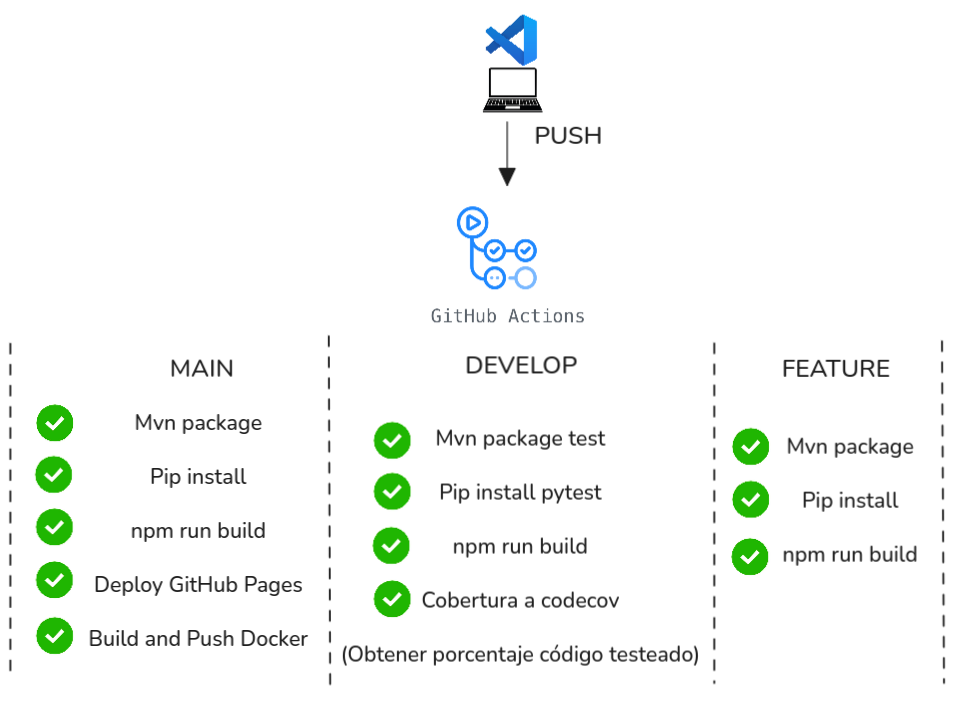
\includegraphics[width=0.8\textwidth]{fotos/githubActions.png}
  \caption{Flujo de desarrollo github actions}
  \label{fig:gitactions}
\end{figure}

\subsubsection*{Workflow para ramas \texttt{feature/*}}

Este workflow se activa con un \texttt{push} a cualquier rama que empiece por \texttt{feature/} y con Pull Requests dirigidos a \texttt{develop}. Las acciones que realiza son: 

\begin{itemize}
  \item Compilación de microservicios en Spring Boot
  \item Instalación de dependencias Python.
  \item Instalación de dependencias Node.js.
  \item Construcción del frontend para validar que no haya errores.
\end{itemize}
\subsubsection*{Workflow para la rama \texttt{develop}}

Este workflow se activa con cada \texttt{push} a la rama \texttt{develop}. Su objetivo principal es ejecutar pruebas automatizadas y medir la cobertura del código. Las acciones que realiza son: 

\begin{itemize}
  \item Configuración del entorno con Ubuntu y Java 17.
  \item Restauración de la caché de dependencias Maven.
  \item Construcción del frontend para validar que no haya errores.
  \item Ejecución de tests en todos los microservicios Java con generación de reportes Jacoco.
  \item Ejecución de tests en Python para microservicios específicos.
  \item Envío de los reportes de cobertura a Codecov \cite{codecov}.
\end{itemize}



\subsubsection*{Workflow para la rama \texttt{main}}

Este workflow se activa al hacer \texttt{push} a la rama \texttt{main} y se centra en realizar el despliegue de la aplicación. Las acciones que realiza son: 

\begin{itemize}
  \item Compilación completa de microservicios Java y construcción de imágenes Docker.
  \item Construcción y despliegue del frontend en GitHub Pages.
  \item Construcción del microservicio en Python.
  \item Login en Docker Hub para subir imágenes Docker de los microservicios Java y Python.
\end{itemize}
\vspace{0.5em}
Además, se ha creado un \href{https://github.com/users/alonsodm12/projects/5}{proyecto en Github}, donde se han definido las historias de usuario y se han organizado en las distintas iteraciones del trabajo. De esta forma, GitHub se ha convertido en la herramienta central para la planificación y el desarrollo.

\begin{figure}[H]
  \centering
  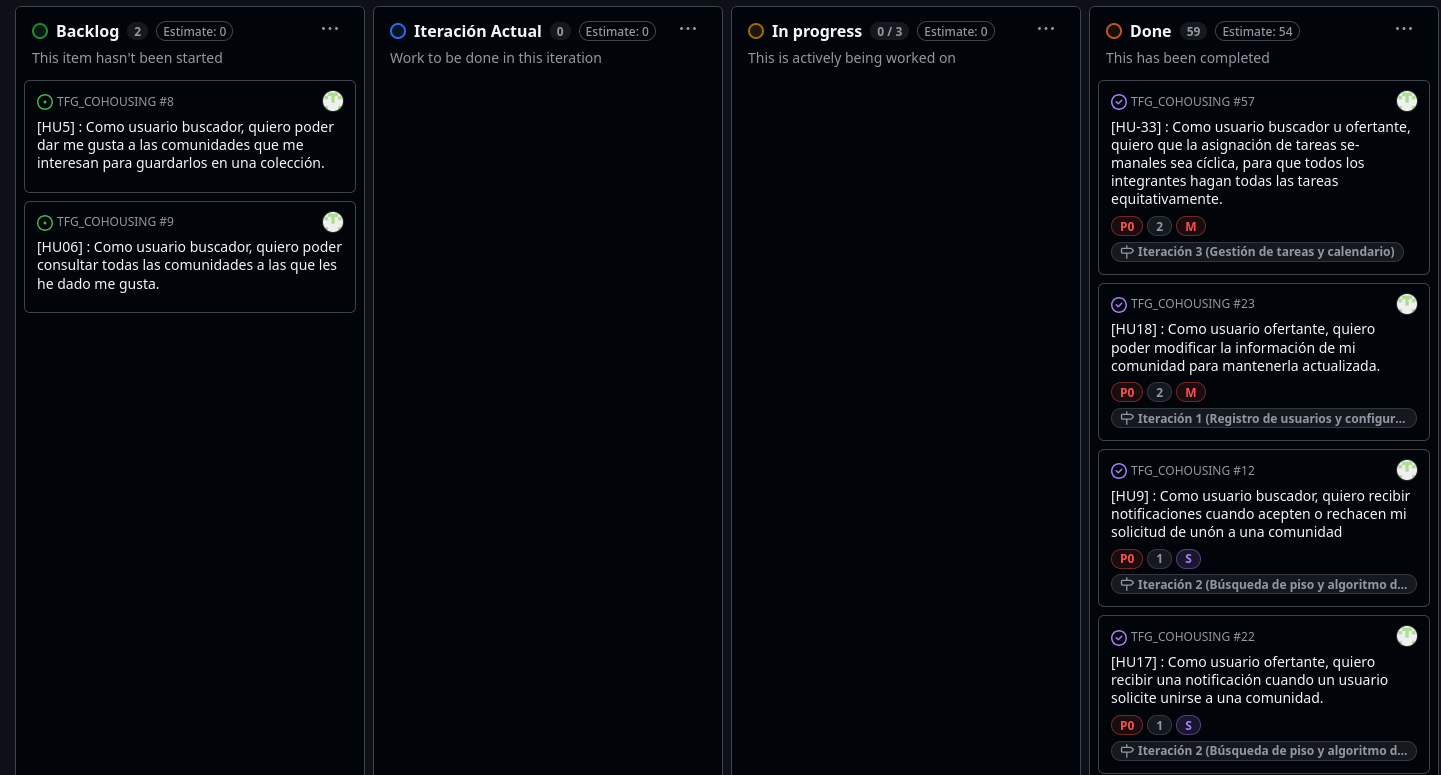
\includegraphics[width=1\textwidth]{fotos/backlog-github.png}
  \caption{Imagen tablero GitHub Project}
\end{figure}

\subsection{Contenerización con Docker}
\begin{figure}[H]
  \centering
  
\includegraphics[width=0.4\textwidth]{fotos/docker.png}
  \caption{Logo docker}
\end{figure}
Cada microservicio y front-end disponen de su propio Dockerfile\cite{docker}, un archivo mediante el cuál se configuran los recursos y dependencias necesarias para su ejecución en un entorno controlado.
Esto permite crear un sistema modular donde cada microservicio se ejecuta de forma aislada en su contenedor específico. 

A continuación se procede a mostrar el ejemplo de configuración de un Dockerfile para los microservicios en Java.
\begin{verbatim}
FROM openjdk:17-jdk-slim
COPY target/demo.jar app.jar
EXPOSE 8081
ENTRYPOINT ["java","-jar","/app.jar"]
\end{verbatim}

Como se puede observar, lo único que se realiza es copiar el .jar del microservicio ya compilado en el contenedor y ejecutarlo. Esta configuración permite desplegar servicios independientes en cualquier entorno compatible con Docker de forma sencilla y efectiva.

\subsection{Orquestación con Docker Compose}

Se emplea un fichero \texttt{docker-compose.yml}\cite{dockercompose} para levantar todo el ecosistema de servicios que componen la aplicación. En general la estructura del archivo es la siguiente
\begin{itemize}
  \item Construcción de microservicios desde sus contextos a partir del DockerFile de cada servicio.
  \item Definición de bases de datos PostgreSQL y servicio RabbitMQ.
  \item Red interna \texttt{cohousing} para comunicación entre contenedores.
  \item Uso de \texttt{depends\_on} para gestionar el orden de arranque.
\end{itemize}

Finalmente para poder ejecutar la aplicación se levanta el entorno completo, esto permite ejecutar en local todos los servicios simultáneamente, para ello se ejecuta el siguiente comando.

\begin{verbatim}
docker-compose up --build
\end{verbatim}

Esta configuración permite una gestión modular, escalable y replicable de la aplicación, facilitando tanto el desarrollo local como el despliegue en entornos de producción.


\section{Funcionalidades clave del sistema}

A continuación se procederá a explicar las diferentes funcionalidades del sistema, mostrando su lógica y flujo de desarrollo.

\subsection{Inicio de sesión y Registro}
Con el objetivo de garantizar la seguridad dentro de la aplicación y asegurar la autenticación y autorización se ha aplicado un sistema de inicio de sesión basado en JWT (JSON Web Token) \cite{jwt}. El flujo de esta funcionalidad es el siguiente: 
 
\begin{itemize}
  \item El usuario envía sus credenciales al \textit{API Gateway}.
  \item El gateway se comunica con el microservicio \textit{Gestión de Usuarios} donde se autentica al usuario y se genera el JWT si las credenciales son correctas.
  \item Este token es enviado al cliente y debe ser adjuntado en el header de las peticiones posteriores para validar la sesión.
  \item En el microservicio \textit{API Gateway}, cada vez que un cliente accede a una ruta protegida, se aplica un filtro personalizado de Spring Security que intercepta la petición y valida la autenticidad del token JWT.
\end{itemize}

\vspace{0.5em}

\begin{figure}[H]
    \centering
    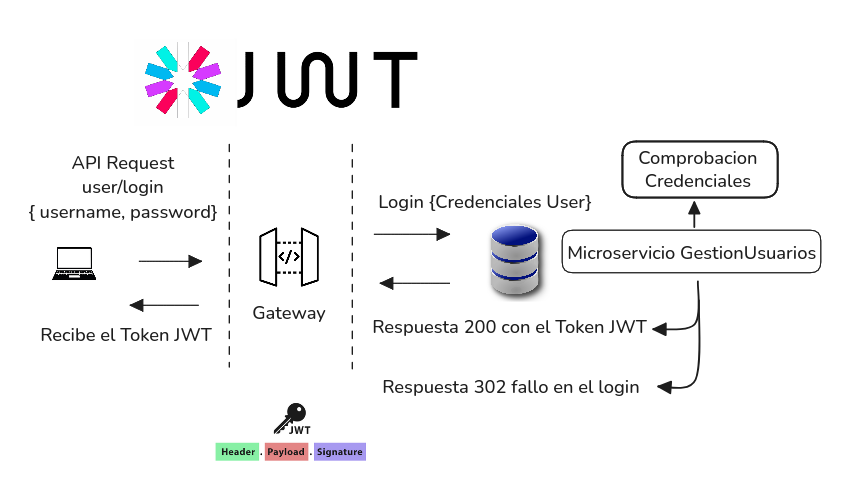
\includegraphics[width=\textwidth]{fotos/jwt_login.png}
    \caption{Flujo de autenticación a través del API Gateway.}
    \label{fig:loginImpl}
\end{figure}

Para implementar el esquema de autenticación basado en JWT representado en la figura \ref{fig:loginImpl}, se han desarrollado los siguientes componentes en la aplicación Spring Boot:
\vspace{0.5em}
\begin{enumerate}[label=\textbf{\arabic*.}]
    \item \textbf{Filtro de seguridad en la API Gateway:} \\
    Se definió un filtro de seguridad que se inserta en la cadena de filtros de Spring Security\cite{springsecurityjwt}. Este filtro es responsable de establecer los requisitos de seguridad correspondientes para cada ruta definida  y de comprobar la validez del token JWT en cada solicitud a una ruta protegida.

    \item \textbf{Generación del token JWT:} \\
    Cuando los datos proporcionados por el usuario durante el proceso de inicio de sesión sean correctos, se procede a generar un token JWT que contiene la información de autenticación del usuario, en nuestro caso el nombre de usuario y el rol.

    \item \textbf{Controlador de autenticación:} \\
    Se definió un controlador REST que gestiona las peticiones de autenticación. Este controlador valida las credenciales del usuario y, en caso de ser válidas, devuelve el token JWT en la respuesta.
\end{enumerate}


\begin{lstlisting}[language=Java, caption={Pseudocódigo del controlador login}]
function login(loginRequestDTO, response):

    try:
        # Intentar autenticar al usuario
        token = authService.login(loginRequestDTO)

        # Guardar el token como cookie de autenticacion
        addAuthCookie(response, token)

        # Obtener el rol del usuario desde el token
        role = tokenService.getRoleFromToken(token)

        # Devolver respuesta de exito con datos del usuario
        return ResponseEntity.ok({
            "message": "Login correcto",
            "username": loginRequestDTO.username,
            "role": role
        })

    except AuthenticationException:
        # Si las credenciales no son validas, devolver error
        return ResponseEntity.status(BAD_REQUEST).body({
            "error": "Credenciales invalidas"
        })
\end{lstlisting}

En el frontend simplemente se rellena el formulario de inicio de sesión, mostrado en la figura \ref{fig:loginFront}, enviándo los datos necesarios para la autenticación.
\begin{figure}[H]
  \centering
  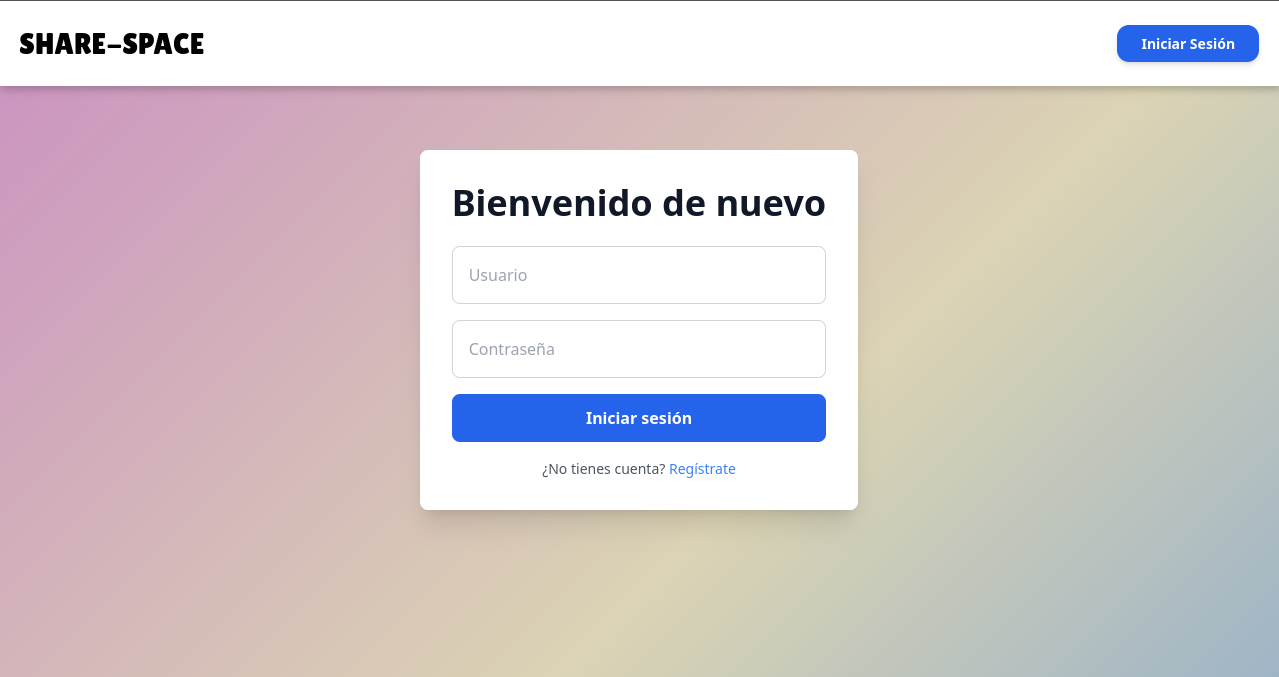
\includegraphics[width=1\textwidth]{fotos/login.png}
  \caption{Pantalla del login en el front-end}
  \label{fig:loginFront}
\end{figure}

Tras iniciar sesión correctamente se accede a la pantalla de inicio, imagen \ref{fig:home}, donde el usuario podrá acceder a toda la funcionalidad desarrollada.
\begin{figure}[H]
  \centering
  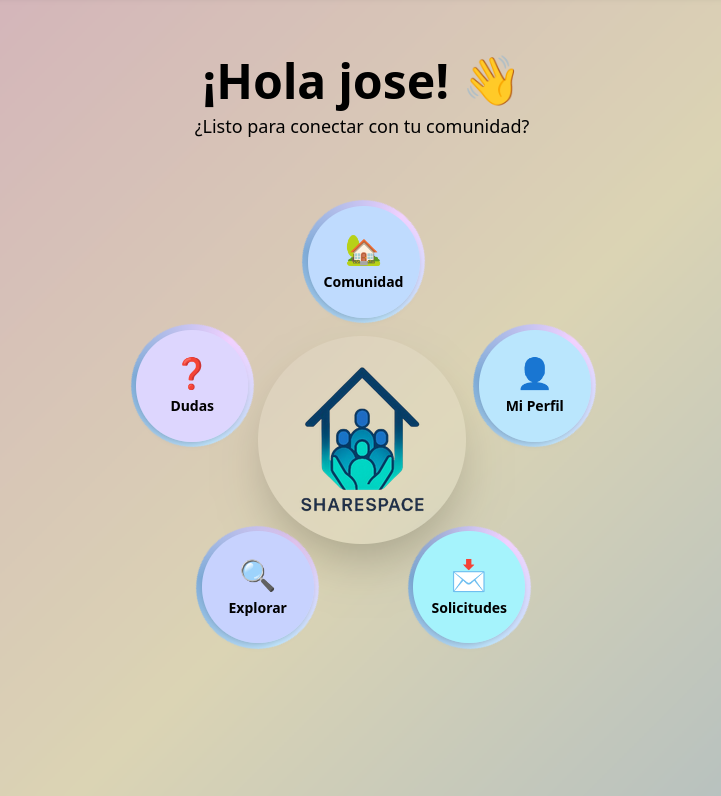
\includegraphics[width=1\textwidth]{fotos/menuOpciones-memoria.png}
  \caption{Pantalla de inicio de la aplicación}
  \label{fig:home}
\end{figure}



\subsection{Comunicación Asíncrona entre Microservicios}

Para garantizar la resiliencia e independencia entre los distintos microservicios que componen el sistema, es fundamental que la comunicación entre ellos sea asíncrona ya que de otra forma podrían producirse cuellos de botella o incluso una caída del sistema entero ante algún fallo en uno de los servicios.
Con el objetivo de implementar este tipo de comunicación, se ha integrado el broker de mensajería asíncrona \textbf{RabbitMQ}, que actúa como intermediario en el intercambio de mensajes entre microservicios.

\subsection*{Flujo de comunicación}

El flujo seguido para establecer esta arquitectura de mensajería es el siguiente:

\begin{itemize}
    \item Los microservicios publican eventos en colas específicas gestionadas por RabbitMQ.
    \item Otros microservicios se suscriben a dichas colas, reaccionando ante los mensajes recibidos.
    \item Esta arquitectura permite reducir el acoplamiento entre los microservicios, consiguiendo una mayor escalabilidad, tolerancia a fallos e independencia entre ellos.
\end{itemize}

\subsection*{Funcionamiento del sistema}

La lógica general de funcionamiento se basa en los siguientes pasos:

\begin{enumerate}[label=\textbf{\arabic*.}]
    \item El microservicio define un evento que producirá una comunicación con otro microservicio, por ejemplo solicitar la unión a una comunidad.
    \item El microservicio productor registra una nueva cola específica en RabbitMQ que estará asociada al evento definido anteriormente.
    \item Al producirse el evento, se crea un mensaje con los datos relevantes y se publica en dicha cola.
    \item Los microservicios consumidores definen \textit{listeners} (funciones observadoras) que se mantienen a la escucha.
    \item Cuando el mensaje llega a la cola correspondiente, el \textit{listener} lo recibe, extrae los datos y ejecuta una lógica específica en respuesta al evento.
\end{enumerate}

Este patrón de comunicación mostrado en la figura \ref{fig:RabbitMQexpl} favorece un diseño desacoplado, reactivo y preparado para entornos distribuidos y de alta disponibilidad.

\begin{figure}[h!]
  \centering
  \includegraphics[width=1\textwidth]{fotos/RabbitMQexpl.png}
  \caption{Flujo de eventos y comunicación entre microservicios usando RabbitMQ}
  \label{fig:RabbitMQexpl}
\end{figure}
\subsection{Recomendación de Comunidades}

Toda la lógica e implementación relacionada con la recomendación de comunidades se ha encapsulado en un microservicio independiente denominado \textbf{Recomendaciones}. Esta decisión se basa en que el módulo presenta suficientes reglas de negocio como para ser considerado una entidad lógica separada dentro del sistema.

\vspace{0.5em}
Para la implementación del microservicio se ha utilizado el lenguaje de programación \textbf{Python}, apoyado en las siguientes bibliotecas:

\begin{itemize}
    \item \texttt{Pandas} \cite{pandas}, para el tratamiento y análisis de datos.
    \item \texttt{FastAPI} \cite{fastapi}, para la creación y estructuración de la API REST.
\end{itemize}

\subsection*{Algoritmo de recomendación}

Con el objetivo de conseguir una recomendación personaliza para cada usuario se ha seguido un enfoque basado en técnicas de \textit{clustering}, mediante el algoritmo \textbf{K-Means} \cite{kmeans}. Esto ha permitido agrupar las comunidades en función de la similitud de sus parámetros de afinidad. Una vez organizados estos grupos, se ha identificado el más cercano al usuario calculando la similitud entre los valores de afinidad del usuario y los de las comunidades de cada grupo. La lógica general del sistema se puede resumir del siguiente modo:


\vspace{0.5em}
\begin{itemize}
    \item Las comunidades se agrupan en \textit{clusters} en función de sus características individuales (afinidad, sociabilidad, limpieza, etc.).
    \item Se entrena un modelo \texttt{KMeans} únicamente con las comunidades.
    \item Se predice a qué \textit{cluster} pertenecería un usuario en base a sus características.
    \item Se seleccionan las comunidades que pertenecen al mismo \textit{cluster} que el usuario.
    \item Se ordenan esas comunidades según su cercanía al vector escalado del usuario, de forma que sea lo más personalizado posible.
\end{itemize}

\subsection*{Procedimiento de recomendación}

Dentro del propio microservicio se ha seguido el siguiente flujo para generar las recomendaciones personalizadas para cada usuario:

\begin{enumerate}[label=\textbf{\arabic*.}]
    \item Se recuperan los datos del usuario objetivo y de las comunidades desde sus respectivas bases de datos.
    \item Se normalizan los parámetros de afinidad tanto del usuario como de las comunidades, esto es necesario para que la distancia euclídea tenga sentido.
    \item Se entrena un modelo de \texttt{K-Means} con los datos escalados de las comunidades.
    \item Se predice a qué \textit{cluster} pertenecería el usuario, para ello se calcula la diferencia (distancia euclídea) entre el vector del usuario y el centroide de cada grupo, que funciona como representación del perfil idea de ese grupo de comunidades.
    \item Se calcula la distancia euclídea entre cada comunidad del mismo \textit{cluster} escogido y el vector escalado del usuario.
    \item Se transforma la distancia en un porcentaje de afinidad (0 a 100).
    \item Las comunidades del clúster se ordenan por mayor afinidad y se seleccionan las \texttt{n} más afines para formar la recomendación.
\end{enumerate}
\vspace{0.5em}

\begin{lstlisting}[language=Python, caption={Pseudocódigo de la función recommend\_communities\_by\_user}]
def recommend_communities_by_user(user, communities, n_recommendations=10):
    
    # Si no hay comunidades, devolvemos la lista vacia
    if communities is None or len(communities) == 0:
        return []

    # Preprocesar y escalar datos, es necesario tener los datos escalados y en un formato correcto para aplicar K-Means
    user_scaled, communities_scaled = preprocess_data(user, communities)

    #Si no hay usuarios, devolvemos error
    if user_scaled is None or communities_scaled is None:
        raise ValueError("Error al escalar los datos")

    # Definimos el numero de clusters que tendremos
    n_clusters = min(3, len(communities_scaled))
    if n_clusters == 0:
        return []

    # Entrenar modelo KMeans
    kmeans = KMeans(n_clusters=n_clusters, random_state=42)
    kmeans.fit(communities_scaled)

    # Predecir cluster del usuario y de las comunidades

    # K-Means nos dice a que cluster pertenece el usuario
    user_cluster = kmeans.predict(user_scaled)[0]

    # K-Means predice en que cluster cae cada comunidad
    # Devuelve un vector indicando en que cluster se encuentra cada comunidad
    communities_clusters = kmeans.predict(communities_scaled)

    # Calculamos el centroide del cluster del usuario
    # El centroide es un vector con las coordenadas medias de ese grupo
    user_center = kmeans.cluster_centers_[user_cluster]

    # Calcular distancias entre las comunidades del cluster escogido y el centroide del usuario
    distances = []
    # Recorremos todas las comunidades
    for i, community_scaled in enumerate(communities_scaled):
        # Solo nos fijamos en aquellas que estan en el mismo cluster que el usuario
        if communities_clusters[i] == user_cluster:
            # Se calcula la distancia euclidea (np.linalg.norm(...)) entre la comunidad[i} y el usuario
            dist = distancia_euclidiana(community_scaled, user_scaled[0])
            #Esto devuelve una lista de pares indicando primero el id de la comunidad y segundo un valor
            #que indica que tan lejos estan de el
            distances.append((i, dist))

    if not distances:
        return []

    # Normalizar distancias para calcular afinidad
    max_distance = max(dist for _, dist in distances)
    if max_distance == 0:
        max_distance = 1

    MIN_AFFINITY = 30
    affinities = []
    for i, dist in distances:
        if dist es finita:
            affinity = 100 * (1 - dist / max_distance)
        else:
            affinity = 0
        # Limitar entre MIN_AFFINITY y 100
        affinity = max(min(affinity, 100), MIN_AFFINITY)
        affinities.append((i, round(affinity)))

    # Ordenar comunidades por afinidad descendente
    affinities.sort(descending by affinity)

    # Construir lista final de recomendaciones
    recommended = []
    for i, affinity in affinities[:n_recommendations]:
        recommended.append(
            community_to_dict(communities[i]) + {"affinity": affinity}
        )

    return recommended
\end{lstlisting}



Este enfoque permite recomendar comunidades al usuario de forma personalizada y priorizando la afinidad entre ambos.

\begin{figure}[H]
  \centering
  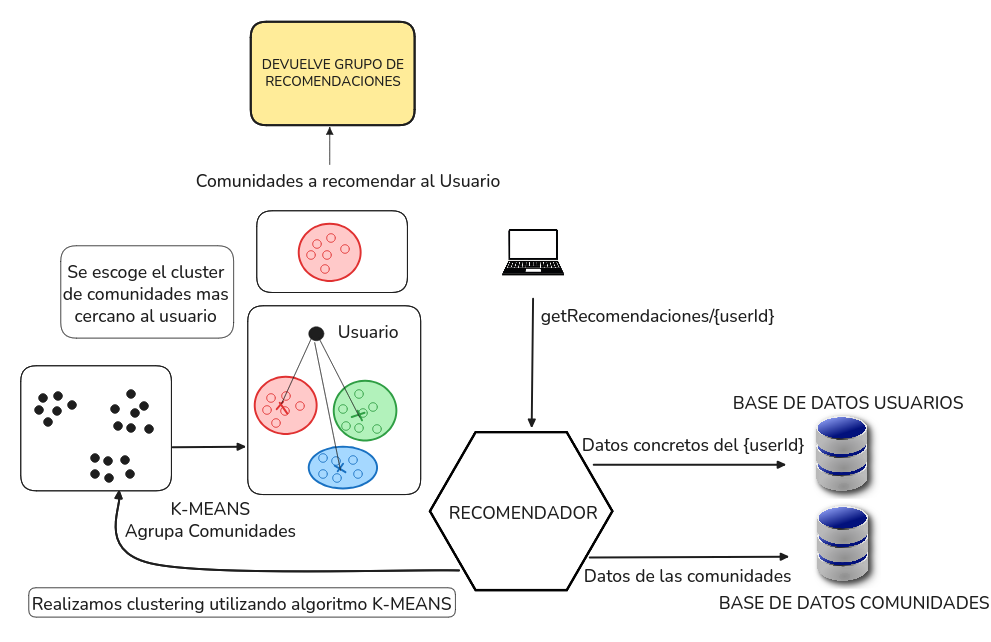
\includegraphics[width=1\textwidth]{fotos/clustering.png}
  \caption{Explicación del sistema de recomendación para usuarios}
  \label{fig:clustering}
\end{figure}
Este sistema de recomendación mostrado en la figura \ref{fig:clustering} es especialmente útil en escenarios de \textit{cold start}, ya que no requiere un historial de interacciones del usuario, sino que se basa en similitud de perfiles.
Cabe destacar que la aplicación permite refinar aún más las recomendaciones de comunidades mediante filtros adicionales, como la distancia al usuario y el rango de precio. Esto proporciona una lista de comunidades más personalizada y ajustada a las preferencias del usuario.

Finalmente, tal como se observa en la figura \ref{fig:frontend-recomendador}, el usuario dispone de opciones para aplicar filtros adicionales y se le muestran las comunidades recomendadas junto a sus datos más representativos.
\vspace{0.5em}
\begin{figure}[H]
  \centering
  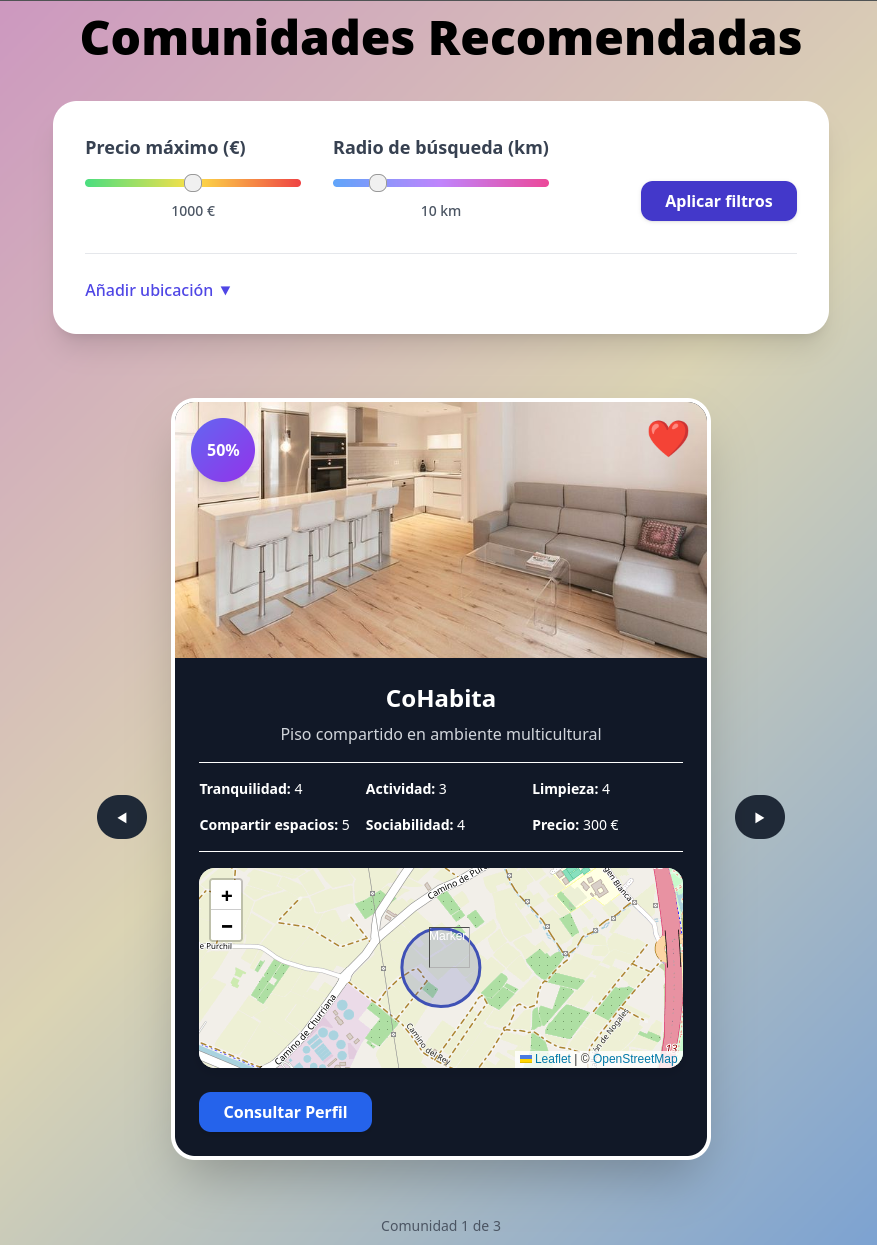
\includegraphics[width=0.8\textwidth]{fotos/frontend-recomendador.png}
  \caption{Pantalla de recomendaciones en el front-end}
  \label{fig:frontend-recomendador}
\end{figure}

\subsection{Proceso de Unión a una Comunidad}

El proceso de unión de un usuario a una comunidad involucra la interacción de varios de los microservicios que componen el sistema, entre ellos los microservicios de \textit{Comunidad}, \textit{Solicitudes} y \textit{GestionUsuarios}.
Para la comunicación entre dichos microservicios se usará como broker RabittMQ \cite{RabbitMQ}. El flujo para realizar esta operación dentro del sistema es el siguiente:

\vspace{0.5em}
\begin{enumerate}
  \item El usuario solicita unirse a una comunidad a través de la llamada al endpoint unirse-comunidad del microservicio \textit{GestionComunidades}.
  \item Este microservicio genera un evento y lo publica en RabbitMQ.
  \item El microservicio de \textit{Solicitudes} escucha el evento, registra la solicitud y la notifica al administrador de la comunidad.
  \item El administrador puede aceptar o rechazar la solicitud mediante el microservicio de \textit{Solicitudes}. Al aceptar o rechazar el microservicio genera un evento y lo publica en RabbitMQ
  \item El microservicio de \textit{GestionComunidades} escucha el evento y si el administrador ha aceptado, une al usuario a la comunidad. Finalmente este microservicio emite un evento y lo publica en RabbitMQ.
  \item El microservicio de \textit{Solicitudes} escucha el evento, registra la respuesta y la notifica al usuario buscador.
\end{enumerate}

\vspace{0.5em}

Este flujo de comunicación entre los diferentes microservicios queda resumido en la figura \ref{fig:union-comunidad}, mostrando como los diferentes microservicios van generando eventos en función del estado de la comunicación actual y como todo el proceso es orquestado por RabbitMQ.

\begin{figure}[H]
  \centering
  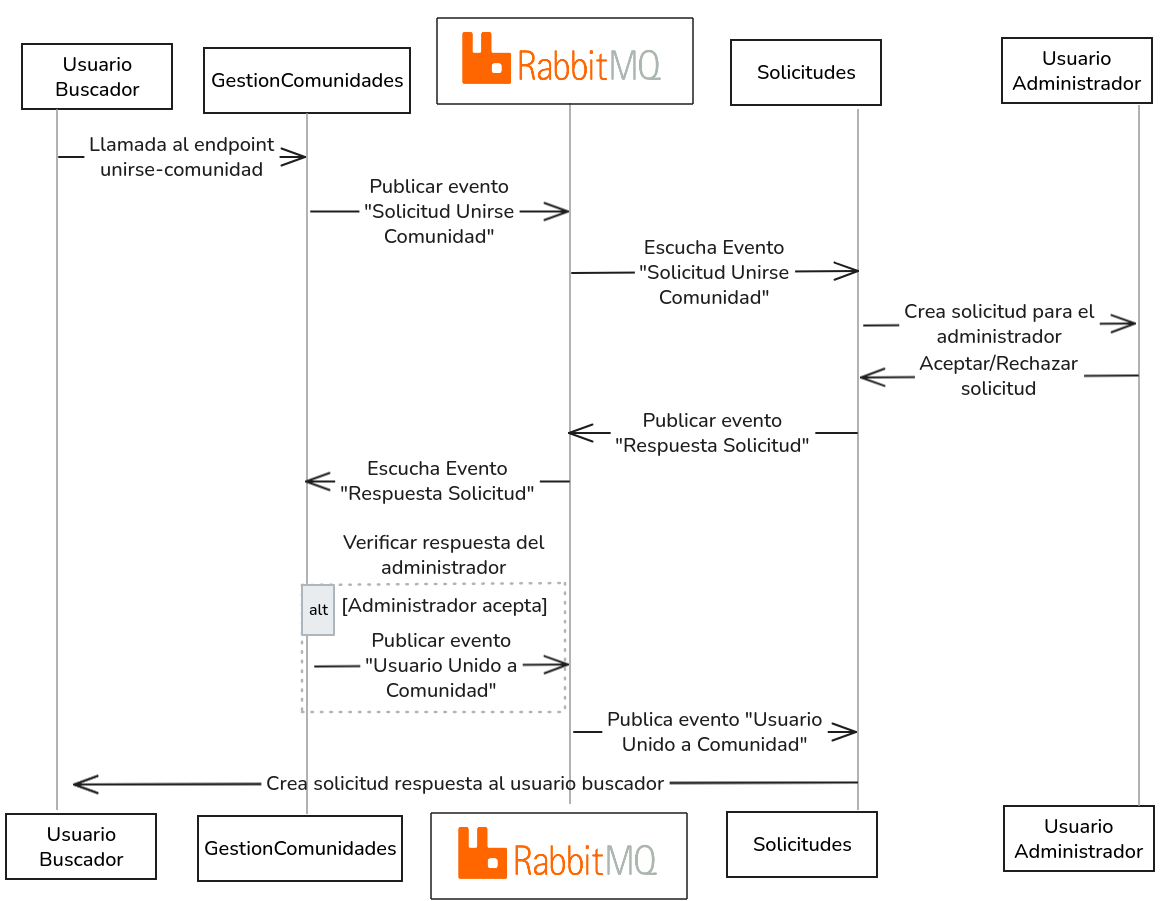
\includegraphics[width=1\textwidth]{fotos/usuarioUneComunidad.png}
  \caption{Esquema del flujo para la unión de un usuario a una comunidad}
  \label{fig:union-comunidad}
\end{figure}





\newpage


\subsection{Gestión de comunidades}
El microservicio de \textbf{Gestión de Comunidades} encapsula el mayor volumen de lógica de negocio dentro del sistema, siendo responsable de coordinar todos los aspectos relacionados con las comunidades: sus eventos, la asignación y la gestión de tareas.

Entre las funcionalidades más relevantes implementadas en este servicio, destacan:

\begin{itemize}
  \item \textbf{Reparto automático de tareas:}  
  El sistema realiza una distribución automática de las tareas entre los usuarios que forman parte de una comunidad, siguiendo un orden cíclico. Este reparto se ejecuta de forma semanal, asegurando así un equilibrio en la carga de trabajo entre los miembros.

  \item \textbf{Administración de tareas por parte del usuario:}  
  Los usuarios tienen la posibilidad de consultar y reorganizar sus tareas mediante una interfaz de calendario interactivo. Esta herramienta permite una gestión más intuitiva y visual de sus responsabilidades.
\end{itemize}
Estas funcionalidades se ofrecen al usuario a través de la interfaz de la comunidad, como se muestra en la figura \ref{fig:comunidad-memoria}.

\begin{figure}[H]
  \centering
  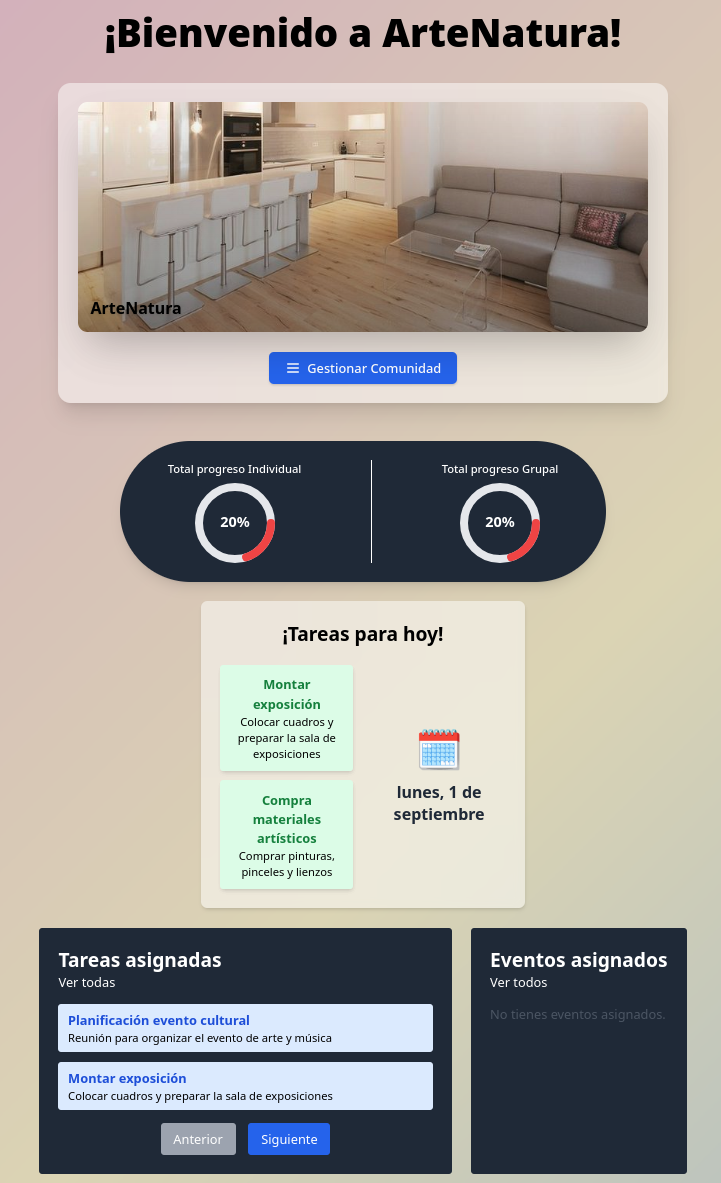
\includegraphics[width=1\textwidth]{fotos/comunidad-memoria.png}
  \caption{Vista de la comunidad del usuario}
  \label{fig:comunidad-memoria}
\end{figure}
\subsection*{Reparto Automático de Tareas}

El reparto automático de tareas tiene como objetivo asegurar una distribución equitativa del trabajo entre los miembros de cada comunidad. Para ello, se sigue un algoritmo cíclico que asigna las tareas disponibles a los usuarios de manera rotativa.

Con este objetivo en mente se ha diseñado el siguiente algoritmo teniendo en cuenta:
\begin{itemize}
  \item El conjunto de usuarios activos en la comunidad.
  \item Las tareas asociadas a la comunidad.
  \item El historial de asignaciones anteriores, para mantener el reparto equitativo.
\end{itemize}

De esta manera, el sistema garantiza una planificación justa y eficiente, mejorando la organización interna de cada comunidad.

\subsection*{Lógica del reparto cíclico}

El reparto de tareas se ha diseñado siguiendo una lógica sencilla pero equitativa. A continuación, se describe el comportamiento implementado:

\begin{itemize}
    \item Las tareas se distribuyen de forma \textbf{cíclica} entre los integrantes de la comunidad. De este modo, con el tiempo, todos los miembros participarán en todas las tareas.
    \item Al crear una nueva tarea, se define el \textbf{número de participantes requeridos}.
    \item En el primer reparto, se asignan por defecto los primeros usuarios disponibles. De forma que, si hay cuatro tareas y tres miembros, se asignará la primera tarea al primer miembro; la segunda, al segundo y así sucesivamente en orden cíclico.
    \item En repartos sucesivos, se utiliza un índice rotativo almacenado en la comunidad para determinar desde qué usuario comenzar la asignación. Este índice se va actualizando con cada tarea para que todos los usuarios participen proporcionalmente en alguna tarea en cada iteración. Si un nuevo usuario se une a la comunidad, se incorpora automáticamente a la lista de usuarios rotativos.
\end{itemize}

\vspace{0.25em}
Para lograr la ejecución de forma semanal del reparto se ha utilizado la anotación \textit{@Scheduled(cron = )}. Con esta anotación podemos ejecutar este método definido en el backend de forma periódica; en nuestro caso cada semana.
\begin{lstlisting}[language=Python, caption={Pseudocódigo de la función repartirTareasSemanalmente}]
@Scheduled(cron = "0 0 23 * * SUN")
@Transactional
def void repartirTareasSemanalmente():
    # Obtener todas las comunidades
    comunidades = obtenerTodasLasComunidades()
    hoy = fechaActual()
    # Iterar sobre cada comunidad
    for comunidad in comunidades:
        
        # Repartir tareas de forma ciclica
        repartirTareasCiclico(comunidad.id)
        
        # Generar resumen semanal
        generarResumenSemanal(comunidad, hoy)

        # Obtener lista de identificadores de usuarios de la comunidad
        idUsuarios = lista(comunidad.integrantes)

        # Crear notificacion de reparto de tareas
        payload = crearNotificacionReparto(
            comunidad.id,
            comunidad.nombre,
            "Se ha realizado el reparto de tareas en tu comunidad",
            idUsuarios
        )

        # Enviar notificacion a la cola de mensajeria (RabbitMQ)
        enviarMensajeCola(
            EXCHANGE_REPARTO_TAREAS,
            ROUTING_KEY_REPARTO_TAREAS,
            payload
        )

\end{lstlisting}


\subsection*{Notificación y visualización}

Para asegurar que los usuarios estén al tanto de sus tareas, el sistema emite notificaciones cuando se realiza el reparto semanal:

\begin{itemize}
    \item De manera semanal se emite una \textbf{notificación automática a todos los integrantes de la comunidad} de forma que se les avise del nuevo reparto. Esto se implementa con la definición de un evento dentro de la función de reparto semanal que es gestionada por RabbitMQ. 
\end{itemize}

Esta notificación es mostrada en la plataforma dentro de la sección de Solicitudes, como se puede ver en la imagen
\ref{fig:solicitudes}
\begin{figure}[H]
  \centering
  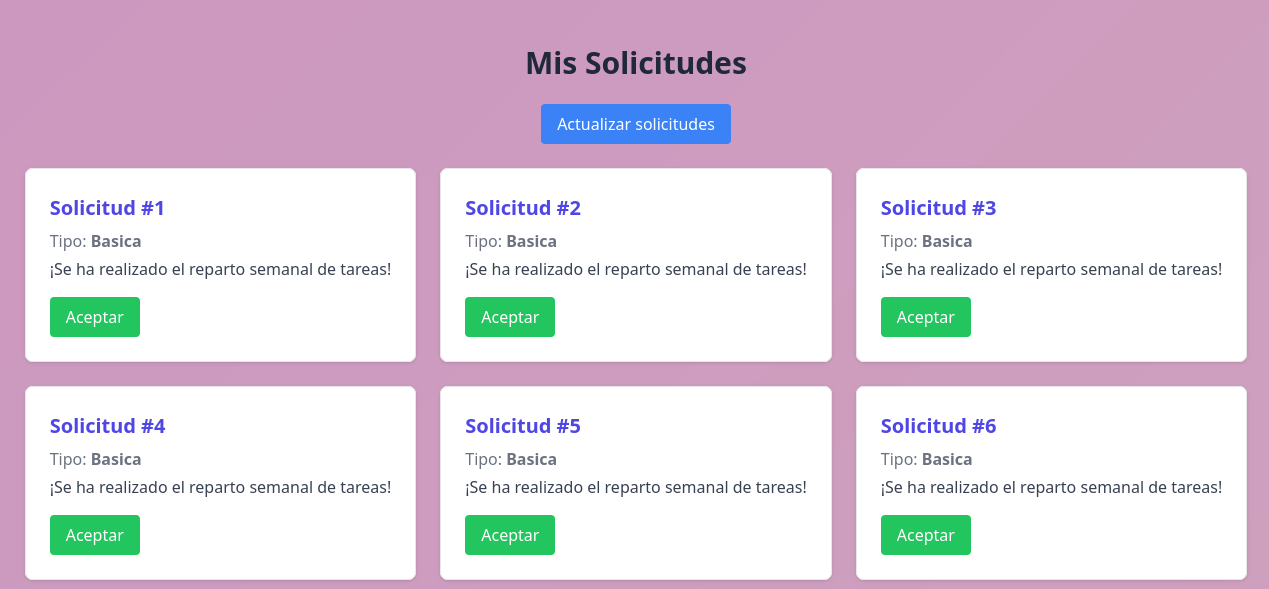
\includegraphics[width=1\textwidth]{fotos/solicitudes-memoria.png}
  \caption{Vista de las solicitudes}
  \label{fig:solicitudes}
\end{figure}

A continuación pasamos a comentar la Administración de tareas por parte del usuario.
\vspace{0.5em}
\subsection{Administración de Tareas por Parte de los Usuarios}

Con el objetivo de facilitar la administración de tareas dentro de la comunidad, se ha desarrollado una interfaz interactiva que permite a los usuarios visualizar, asignar y reprogramar sus tareas mediante un calendario dinámico.

Buscando la mejor experiencia de usuario posible, se ha implementado una funcionalidad de \textit{drag and drop} (arrastrar y soltar), que permite al usuario mover las tareas a diferentes franjas horarias en el calendario, asignándoles así una fecha y hora de inicio de forma intuitiva.

El flujo de funcionamiento del componente es el siguiente:

\vspace{0.5em}
\begin{enumerate}
  \item \textbf{Carga de las tareas del usuario:}  
  En primer lugar, se obtienen todas las tareas correspondientes al usuario mediante el \textit{endpoint} \texttt{/tareas/{idUsuario}}.  
  \begin{itemize}
    \item Las tareas que no tienen fecha asignada se muestran en una columna lateral para ser planificadas por el usuario.
    \item Las tareas ya planificadas se adaptan al formato requerido por la biblioteca \texttt{FullCalendar} \cite{fullcalendar-docs}(\texttt{id}, \texttt{title}, \texttt{start}) y se representan directamente en el calendario.
  \end{itemize}

  \item \textbf{Funcionalidad Drag and Drop:}  
  Las tareas sin fecha se convierten en elementos arrastrables mediante la clase \texttt{Draggable} de \texttt{FullCalendar}. Esto permite al usuario arrastrar una tarea desde la columna lateral y soltarla en una franja del calendario.

  \item \textbf{Asignación de fecha al soltar la tarea:}  
  Cuando el usuario suelta una tarea sobre el calendario, se ejecuta el método \texttt{handleReceive}. Este método extrae el \texttt{id} de la tarea y la fecha seleccionada, y envía esta información al \texttt{backend} mediante el método \texttt{updateTarea} para registrar la nueva fecha.

  \item \textbf{Reprogramación de tareas:}  
  Si el usuario mueve una tarea ya planificada a una nueva franja horaria dentro del calendario, se ejecuta el método \texttt{handleEventDrop}, el cual recalcula la nueva fecha y la actualiza en el \texttt{backend}.
\end{enumerate}
\newpage
\begin{lstlisting}[language=Java, caption={Pseudocódigo de tareas drag and drop y asignacion fecha al soltar tarea}]
function drag and drop(tareasSinFecha):

    # Obtener el elemento contenedor de tareas externas
    draggableEl = getElementById("external-tasks")

    # Verificar si existe y si aun no ha sido inicializado
    if draggableEl != null AND draggableEl._draggableInitialized == false:

        # Crear un nuevo objeto Draggable sobre el contenedor
        # De esta forma todo lo contenido en el contenedor con item fc-task es arrastrable
        new Draggable(draggableEl, {
            itemSelector: ".fc-task",
            eventData: (el) => {
                id = el.getAttribute("data-id") OR ""
                title = el.getAttribute("data-title") OR el.textContent OR ""
                return { id, title }
            }
        })

        # Marcar el elemento como inicializado
        draggableEl._draggableInitialized = true


function asignacion fecha al soltar tarea(info):
    # Esta funcion se ejecuta cada vez que se suelta una tarea en una celda del calendario 

    # Obtener id de la tarea arrastrada
    id = info.event.id

    # Calcular la nueva fecha con ajuste de +2 horas
    if info.event.start != null:
        fecha = toISOString(info.event.start + 2 horas).slice(0,19)
    else:
        fecha = ""

    try:
        # Actualizar fecha de la tarea en el backend
        updateDateTarea(id, fecha)

        # Eliminar la tarea de la lista sin fecha
        setTareasSinFecha( tareasSinFecha.filter(t -> t.id != id) )

        # Agregar la tarea a la lista con fecha
        setTareasConFecha( tareasConFecha + { id, title: info.event.title, start: fecha })

    catch error:
        # En caso de error revertir el drag and drop
        log(error)
        info.revert()
\end{lstlisting}

Gracias a esta implementación, se ha creado una vista de administración de tareas (figura \ref{fig:admin-tareas}) que permite al usuario gestionarlas de forma dinámica. Desde esta interfaz se puede tanto planificar las tareas por primera vez como reorganizarlas posteriormente.
\begin{figure}[h!]
  \centering
  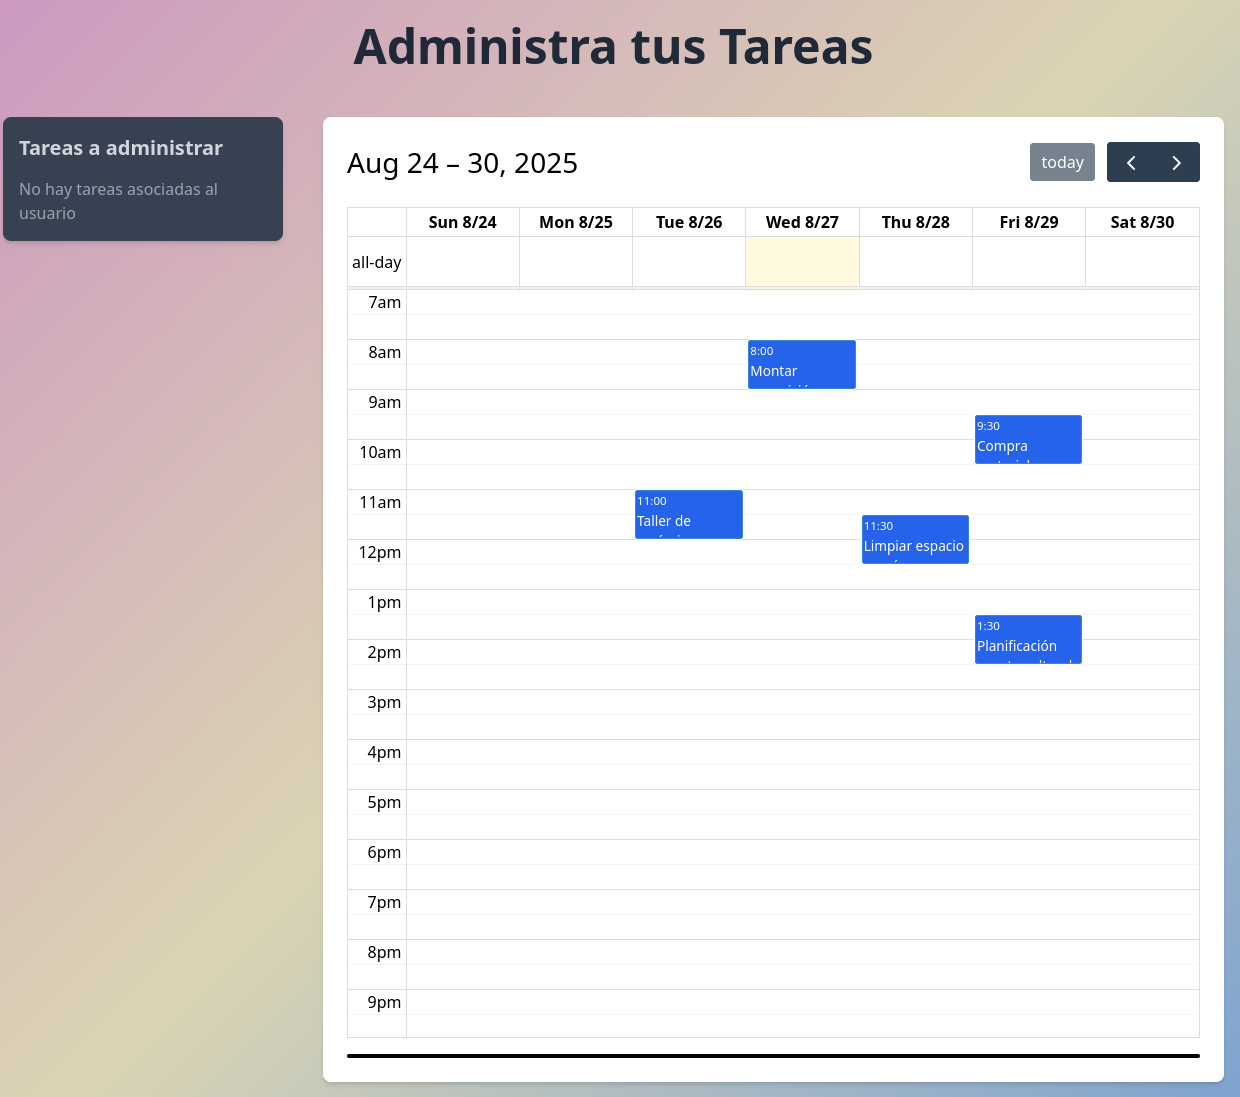
\includegraphics[width=1\textwidth]{fotos/admi-tareas.png}
  \caption{Vista del usuario para la administración de tareas dinámicamente}
  \label{fig:admin-tareas}
\end{figure}
    \chapter{Pruebas} \label{pruebas}

En este capítulo se describen las pruebas realizadas sobre los distintos microservicios que componen la aplicación, así como sobre el frontend. Estas pruebas serán esenciales para asegurar la calidad del software, detectar errores antes de llegar a estados más avanzados y garantizar un comportamiento estable. 

Además, se han integrado en el flujo de integración continua (CI) a través de las GitHub Actions, de manera que se ejecutan automáticamente en cada \textit{subida} a las ramas del repositorio. De este modo, las pruebas forman parte activa del ciclo de vida del desarrollo.

\vspace{0.5em}

Para cada componente se han definido distintos tipos de pruebas con el objetivo de cubrir tanto la lógica individual como el comportamiento global del sistema:

\begin{enumerate}
    \item \textbf{Pruebas Unitarias}: Verifican el comportamiento de clases y funciones de forma aislada, utilizando mocks para simular dependencias externas. Se emplean principalmente JUnit y Mockito para los servicios en Spring Boot, Pytest para los microservicios en Flask y Jest \cite{Jest} con React Testing Library para el frontend.
    
    \item \textbf{Pruebas de Sistema (End to End)}: Validan flujos completos que implican a varios componentes del sistema, especialmente los endpoints más críticos.
    
    \item \textbf{Pruebas de Widgets (Frontend)}: Evalúan la interacción de los elementos de la interfaz de usuario, garantizando su correcto comportamiento frente a las acciones del usuario.
\end{enumerate}

\section{Microservicio de Gestión de Usuarios}

\subsection{Pruebas Unitarias}
Se han probado los siguientes métodos de la capa de servicio:
\begin{itemize}
    \item \texttt{registrarUsuario(UserDTO dto)}: Verifica el registro de un nuevo usuario comprobando si el usuario o alguno de sus datos no han sido previamente registrados. En caso contrario, lanza una excepción controlada.
    \item \texttt{getUsuarioPorId(Long id)}: Comprueba la correcta recuperación de un usuario existente por ID. También se verifica el caso de error mediante una excepción.
    \item \texttt{getComunidadesGuardadas(Long userId)}: Comprueba que se recuperan correctamente las comunidades guardadas por un usuario, incluyendo el caso en que la lista esté vacía.
\end{itemize}

\subsection{Pruebas End to End}
\begin{itemize}
    \item \texttt{POST /user/login}: Se comprueba que con credenciales válidas se obtiene un JWT en la respuesta. También se prueba el caso de credenciales inválidas.
    \item \texttt{GET /user/\{id\}}: Verificación de que se devuelve la información del usuario correspondiente, y se maneja correctamente el caso de ID inexistente.
    \item \texttt{PUT /user/\{id\}}: Se prueba la actualización de datos del usuario y que los cambios se persisten correctamente en la base de datos.
\end{itemize}

Los test han sido pasados todos correctamente, cómo se puede ver en la imagen \ref{fig:test-result}
\begin{figure}[H]
  \centering
  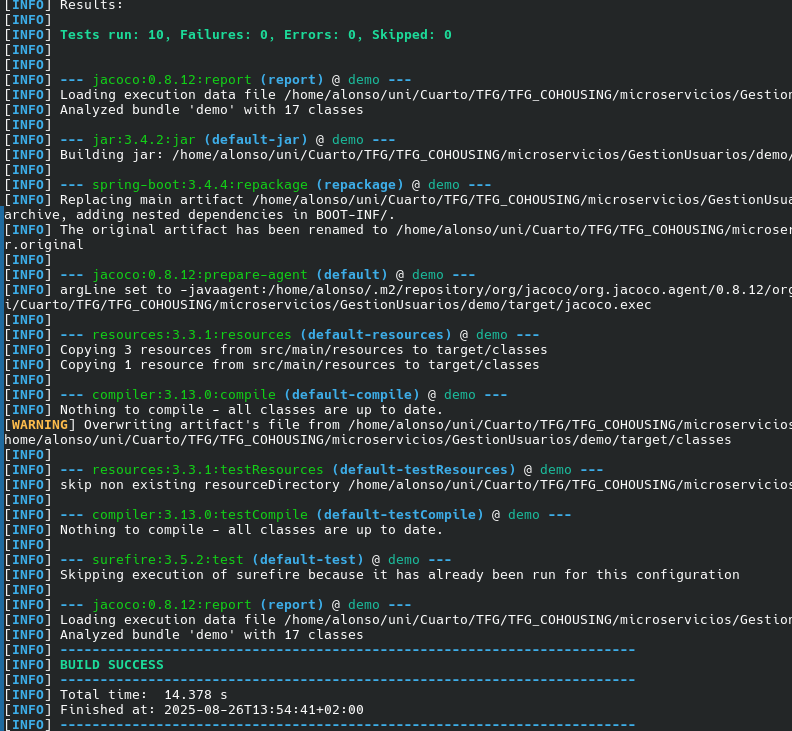
\includegraphics[width=1\textwidth]{fotos/resultadotest-micro-GestionUsuarios.png}
  \caption{Muestra del resultado de los test del microservicio Gestión de Usuarios}
  \label{fig:test-result}
\end{figure}
\section{Microservicio de Gestión de Comunidades}
Este microservicio contiene la lógica central del sistema, especialmente en cuanto a tareas colaborativas y reparto de responsabilidades.

\subsection{Pruebas Unitarias}
\begin{itemize}
    \item \texttt{encontrarPorNombre(String name)} y \texttt{encontrarPorId(Long id)}: Verificación de la recuperación correcta de comunidades por nombre o ID.
    \item \texttt{crearComunidad(CommunityDTO dto)}: Se prueba la creación de comunidades, validando que no exista ya una con el mismo nombre.
    \item \texttt{asignarTareasSemanales()}: Se comprueba que el algoritmo de reparto automático semanal de tareas se ejecuta de forma correcta y equilibrada.
    \item \texttt{addTareaAComunidad(Long communityId, TaskDTO dto)} y \texttt{addEventoAComunidad(Long communityId, EventDTO dto)}: Validación de la correcta asociación de tareas y eventos a una comunidad.
\end{itemize}

\begin{lstlisting}[language=Java, caption={Pseudocódigo del test crearComunidad}]
test "crear comunidad" {
    // Creamos una comunidad falsa
    lifestyleDTO = new LifestyleDTO(1,1,1,1,1)
    dto = new CommunityDTO(
        id = 1L,
        name = "EcoWarning",
        description = "Comunidad preocupada con el medio ambiente",
        ownerId = 7L,
        lifestyle = lifestyleDTO,
        members = [1L, 4L],
        imageUrl = "https://foto",
        latitude = 40.423,
        longitude = 3.45,
        address = "Calle Falsa",
        price = 300.45,
        capacity = 2
    )

    // Mock: metodo para guardar la nueva comunidad 
    mock communityRepository.save(any Community)
        -> devuelve la misma Comunidad pasada

    // Probamos el metodo registrarComunidad
    comunidad = communityService.registrarComunidad(dto)

    // Comprobamos que la comunidad guardada tiene el nombre de la comunidad nueva registrada
    assert comunidad.getName() == "EcoWarning"
}
\end{lstlisting}
\subsection{Pruebas End to End}
\begin{itemize}
    \item \texttt{POST /community/\{id\}/unir}: Verifica que un usuario puede unirse correctamente a una comunidad.
    \item \texttt{GET /community/\{id\}/tasks}: Comprueba la obtención de tareas para su posterior planificación.
    \item \texttt{DELETE /community/\{id\}}: Se prueba la eliminación completa de una comunidad y la cascada de datos relacionada.
\end{itemize}

\section{Microservicio Recomendador}
Este microservicio ha sido implementado con Flask y probado mediante \texttt{pytest}.

\subsection{Pruebas Unitarias}
\begin{itemize}
    \item \texttt{obtener\_todas\_comunidades()}: Verifica que se recuperan correctamente todas las comunidades desde la base de datos.
    \item \texttt{get\_usuario\_perfil(user\_id)}: Prueba la obtención del perfil completo del usuario.
    \item \texttt{recomendar\_comunidades(UserDTO dto)}: Valida que el algoritmo de recomendación devuelve resultados coherentes según los intereses y preferencias del usuario.
\end{itemize}

\subsection{Pruebas End to End}
\begin{itemize}
    \item \texttt{GET /recomendaciones}: Comprueba que se devuelven comunidades recomendadas al usuario autenticado.
    \item \texttt{GET /recomendaciones-filtradas?filtro=\dots}: Se valida que los filtros personalizados funcionan correctamente y modifican los resultados retornados.
\end{itemize}


\begin{lstlisting}[language=Python, caption={Pseudocódigo del test recomendacionesFiltradas}]
test "recomendaciones filtradas" {
    // Se carga el usuario falso creado para las pruebas
    usuario = test_user
    user_id = usuario.id
    
    // Se define parametros de precio y distancia para el filtro
    parametros = {
        "precio": 400,
        "distancia": 5   # 5 km de radio
    }

    // Mock: get_usuario_por_id devuelve el usuario de prueba
    // Mock: get_comunidades_incompletas devuelve comunidades de prueba
    mock get_usuario_por_id -> usuario
    mock get_comunidades_incompletas -> test_communities

    // Se realiza la llamada al endpoint
    respuesta = client.get("usuarios/recomendaciones-filtradas/{user_id}", params=parametros)

    // Se realizan las comprobaciones de la respuesta del endpoint
    assert respuesta.status_code == 200
    datos = respuesta.json()
    assert len(datos) == 1                  // Solo una comunidad
    assert datos[0]["name"] == "Comunidad Cerca"
}
\end{lstlisting}

\section{Microservicio API Gateway}

\subsection{Pruebas Unitarias}
\begin{itemize}
    \item \texttt{extraerToken(HttpHeaders headers)}: Valida que el token JWT es correctamente extraído del encabezado \texttt{Authorization}.
    \item \texttt{validarToken(String token)}: Comprueba que el token es válido y no ha expirado.
\end{itemize}

\begin{lstlisting}[language=Java, caption={Pseudocódigo del test \texttt{validarToken} en \texttt{GatewayServiceTest}}]
test "validarToken" {
  // En primer lugar creamos un mock de los servicios que intervienen en la prueba
  mock JwtUtil, GatewayFilterChain, ServerWebExchange, ServerHttpRequest, ServerHttpResponse, HttpCookie
  
  cookie.value = "tokenValido"
  request.cookies["auth-token"] = cookie
  exchange.request = request
  exchange.response = response
  jwtUtil.validate("tokenValido") -> true
  chain.filter(exchange) -> empty

  // Realizamos la llamada al metodo a probar JwtAuthenticationFilter 
  result = JwtAuthenticationFilter(jwtUtil).filter(exchange, chain)

  // Comprobaciones finales
  expect(result).completes()
  verify(chain.filter(exchange)).calledOnce()
  verify(response.setComplete()).neverCalled()
}
\end{lstlisting}



\subsection{Pruebas End to End}
\begin{itemize}
    \item Se verifica que las peticiones entrantes se enrutan correctamente hacia los microservicios destino según el path y el método HTTP.
\end{itemize}

\section{Microservicio de Solicitudes}

\subsection{Pruebas Unitarias}
\begin{itemize}
    \item \texttt{getSolicitudesUsuario(Long userId)}: Valida que se obtienen todas las solicitudes activas del usuario.
    \item \texttt{deleteSolicitudes(Long userId)}: Prueba que se eliminan correctamente todas las solicitudes del usuario.
    \item \texttt{aceptarSolicitudUnion(Long solicitudId)}: Verifica el cambio de estado de la solicitud a Aceptada.
\end{itemize}
\begin{lstlisting}[language=Java, caption={Pseudocódigo del test aceptarSolicitudUnion}]
test "Aceptar Solicitud Union" {
    
    // Preparar datos de prueba
    solicitudId = 1
    solicitud = crearSolicitud(
        id = solicitudId,
        userOrigenId = 10,
        communityId = 20
    )

    // Mock: al buscar la solicitud, devolver el objeto creado
    mock(solicitudesRepository.findById(solicitudId)).returns(Optional.of(solicitud))

    // Ejecutar la funcion a probar
    response = solicitudesService.aceptarSolicitudUnion(solicitudId)

    // Verificar la respuesta HTTP
    assert response.statusCode == OK
    assert "Solicitud aceptada" en response.body

    // Verificar que se envio un mensaje a RabbitMQ
    verify(rabbitTemplate.convertAndSend(
        EXCHANGE_NAME,
        "comunidad.response",
        cualquierObjeto(UnionResponseDTO)
    ), veces=1)

    // Verificar que la solicitud fue eliminada del repositorio
    verify(solicitudesRepository.deleteById(solicitudId), veces=1)
}
\end{lstlisting}
\subsection{Pruebas End to End}
\begin{itemize}
    \item \texttt{GET /solicitudes/\{id\}}: Se obtiene la solicitud específica en función de Id.
    \item \texttt{GET /solicitudes/usuario/\{id\}}: Devuelve las solicitudes asociadas al usuario.
\end{itemize}


\section{Frontend}

Para las pruebas del frontend, desarrollado en \texttt{React} con \texttt{TypeScript}, se han utilizado las bibliotecas \texttt{React Testing Library} y \texttt{Jest}.

\subsection{Pruebas de Componentes}
\begin{itemize}
    \item Componente de comunidades recomendadas: Verifica que se renderizan correctamente los elementos y que los botones de acción funcionan como se espera.
    \item Componente de detalles de comunidad: Comprueba que los datos se cargan correctamente y que los botones permiten unirse o abandonar una comunidad.
    \item Panel de inicio: Se prueba la carga condicional del contenido según el rol del usuario (administrador, miembro) y su pertenencia a una comunidad.
    \item Solicitudes: Se valida que se visualizan y actualizan correctamente las solicitudes activas del usuario.
\end{itemize}

\begin{lstlisting}[language=Java, caption={Pseudocódigo del test de visualización y actualización de solicitudes}]
test "Mostrar Solicitudes"{
    
    // Mockear la API para devolver solicitudes de prueba
    mock(getSolicitudesUsuario(userId=123)).returns([
        { id: 1, tipo: "compleja", descripcion: "Solicitud de prueba 1" },
        { id: 2, tipo: "basica", descripcion: "Solicitud de prueba 2" }
    ])
    mock(aceptarSolicitud, rechazarSolicitud, eliminarSolicitud).returns({})

    // Renderizar la pagina con MemoryRouter
    render(SolicitudesPage, route="/solicitudes/123")

    // Comprobar que las solicitudes aparecen
    assert screen.findByText("Solicitud #1") exists
    assert screen.findByText("Solicitud de prueba 1") exists
    assert screen.findByText("Solicitud #2") exists
    assert screen.findByText("Solicitud de prueba 2") exists
}
test "Actualizar Solicitudes"{
    
    // Renderizar la pagina con MemoryRouter
    render(SolicitudesPage, route="/solicitudes/123")

    // Seleccionar y clickar el boton de actualizar
    updateButton = screen.getByRole("button", name="Actualizar solicitudes")
    fireEvent.click(updateButton)

    // Verificar que la primera solicitud sigue visible
    assert screen.findByText("Solicitud #1") exists
}
\end{lstlisting}
\section{Ejecución y Cobertura de Pruebas}
Gracias a la integración de las pruebas en el flujo de CI mediante GitHub Actions, estas se ejecutan automáticamente tras cada cambio. Como resultado:

\begin{itemize}
    \item Se asegura que cualquier modificación del código no rompa funcionalidades existentes.
    \item Se generan informes automáticos de cobertura de código mediante Codecov.
    \item Se garantiza que el desarrollo sigue un enfoque orientado a la calidad desde sus primeras etapas.
\end{itemize}

A continuación, se muestra una captura del informe de cobertura generado tras un merge exitoso a la rama \textbf{develop}, imagen \ref{fig:codecov}, se puede observar que el porcentaje de código cubierto tras los test realizados es del 42 por ciento. 

\begin{figure}[h!]
  \centering
  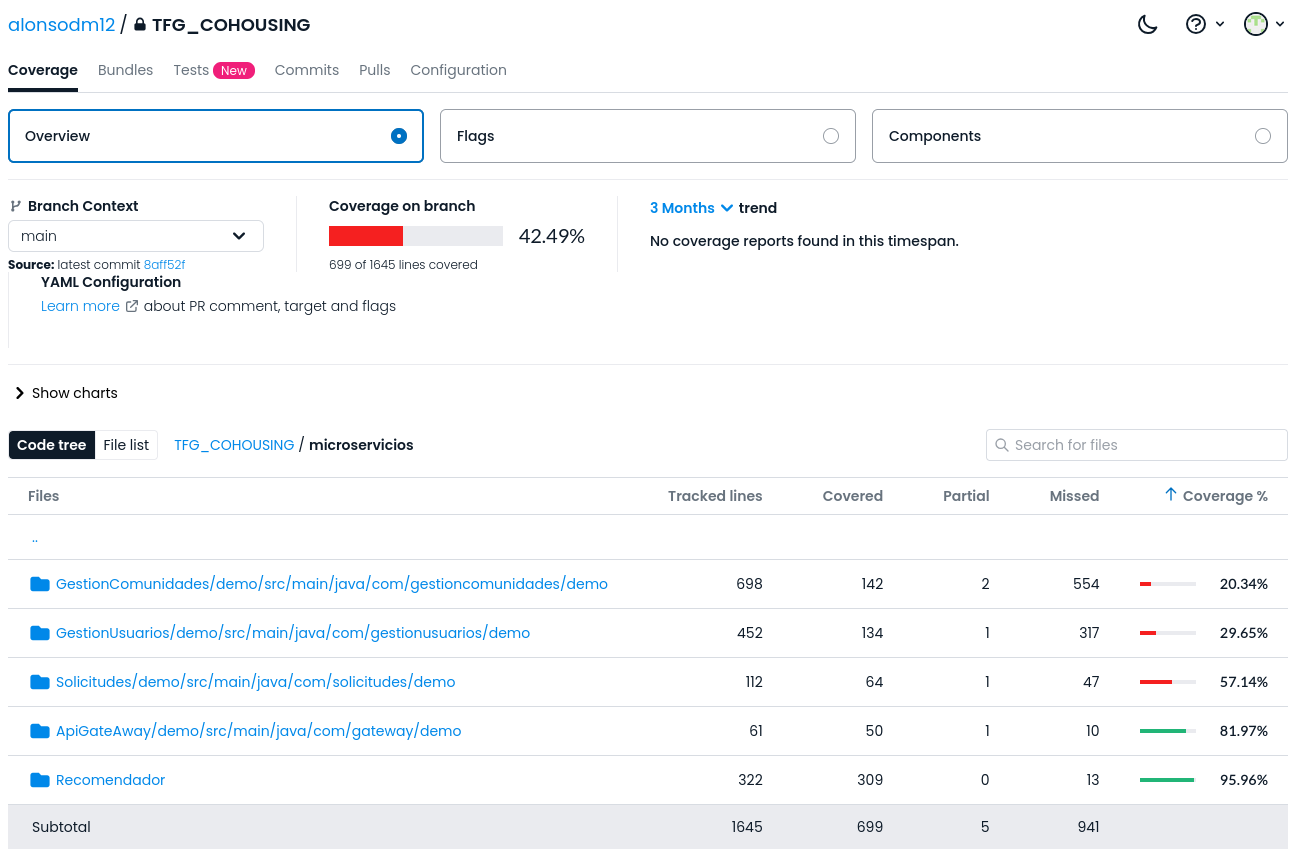
\includegraphics[width=1\textwidth]{fotos/codecov-coverage.png}
  \caption{Muestra del informe de cobertura por Codecov}
  \label{fig:codecov}
\end{figure}

    \chapter{Despliegue} \label{despliegue}

En este capítulo se va a proceder a explicar los pasos seguidos para realizar el despliegue en la nube de la aplicación. Para ello se han utilizado dos plataformas diferentes: \textbf{Github Pages}, que ha permitido desplegar el frontend y \textbf{Railway} \cite{Railway} dónde se han desplegado los 5 microservicios, las tres bases de datos PostgreSQL y un servicio de Rabbitmq. A continuación, se va a mostrar cómo se han realizado ambos despliegues.

\section{Despliegue del frontend}
\begin{figure}[H]
  \centering
  
\includegraphics[width=0.6\textwidth]{fotos/pages.jpg}
  \caption{Logo Github Pages}
  \label{fig:pages}
\end{figure}
Para el despliegue del frontend se ha utilizado la plataforma \textbf{GitHub Pages}, una herramienta gratuita que ofrece GitHub para desplegar sitios estáticos. En nuestro caso, se trata de un proyecto React compilado. 

El procedimiento seguido consiste en:

\begin{enumerate}
    \item Instalar en el proyecto React la dependencia \texttt{gh-pages} mediante el comando:
    \begin{verbatim}
    npm install --save-dev gh-pages
    \end{verbatim}
    
    \item Configurar la variable \texttt{homepage} en el archivo \texttt{package.json} para indicar la URL de despliegue.
    
    \item Ejecutar el comando:
    \begin{verbatim}
    npm run deploy
    \end{verbatim}
\end{enumerate}

Para integrar este proceso dentro del flujo de desarrollo de la aplicación, el frontend se ha desplegado automáticamente cada vez que se realizaba un \textbf{merge} a la rama \texttt{main} (equivalente a producción), gracias a una acción específica configurada en \textbf{GitHub Actions}. 

Finalmente, para que el frontend pueda realizar las llamadas correspondientes tanto en local como en producción, se han configurado una serie de archivos de entorno (\texttt{.env}) que determinan la ruta de consulta correcta en cada caso.

\vspace{0.25em}
Enlace al frontend desplegado: \href{https://alonsodm12.github.io/TFG_COHOUSING/}{Share-Space}


\section{Despliegue del backend}

\begin{figure}[H]
  \centering
  
\includegraphics[width=1\textwidth]{fotos/railway.png}
  \caption{Logo Railway}
  \label{fig:railway}
\end{figure}
Para el despliegue del backend se ha utilizado Railway, un PaaS(Platform as a Service) en la nube que facilita el despliegue de servicios directamente desde repositorios de GitHub, Dockerfiles o plantillas de servicios.

Dentro de Railway se han definido dos proyectos independientes, imagen \ref{fig:railway1} e imagen \ref{fig:railway2}, en los que se han desplegado los distintos servicios que componen el sistema.

\begin{figure}[H]
  \centering
  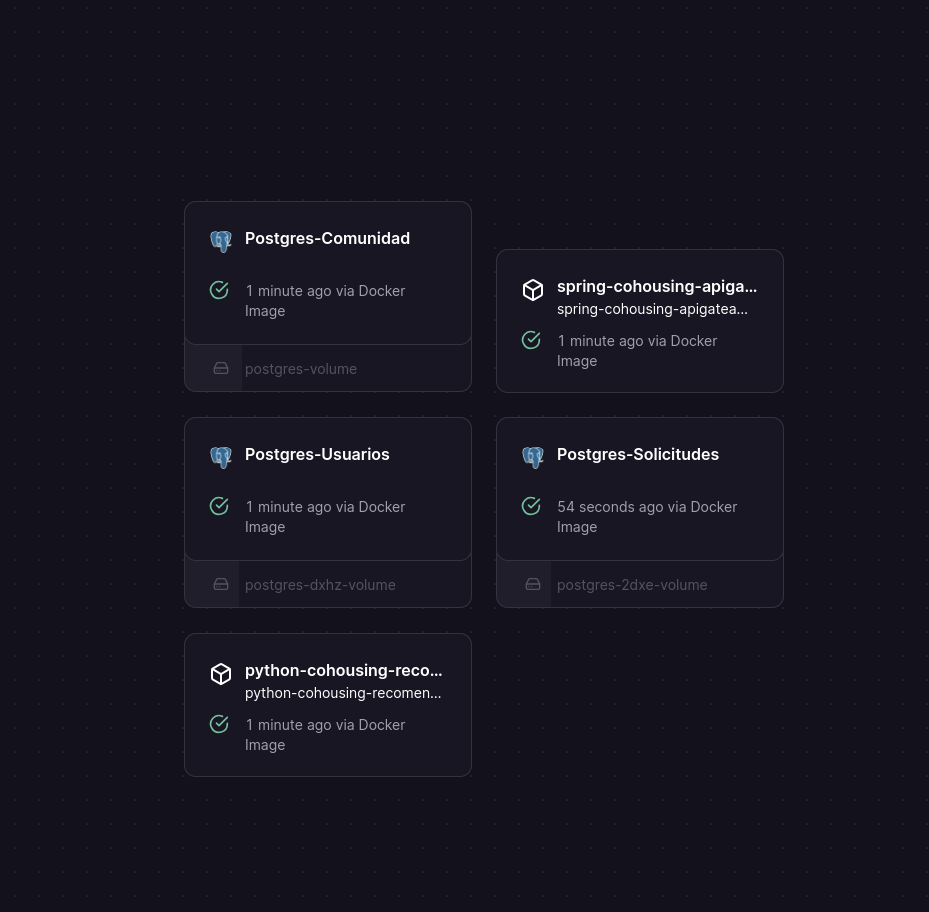
\includegraphics[width=1\textwidth]{fotos/railway1.png}
  \caption{Muestra del tablero de despliegue del primer proyecto en Railway}
  \label{fig:railway1}
\end{figure}


\begin{figure}[H]
  \centering
  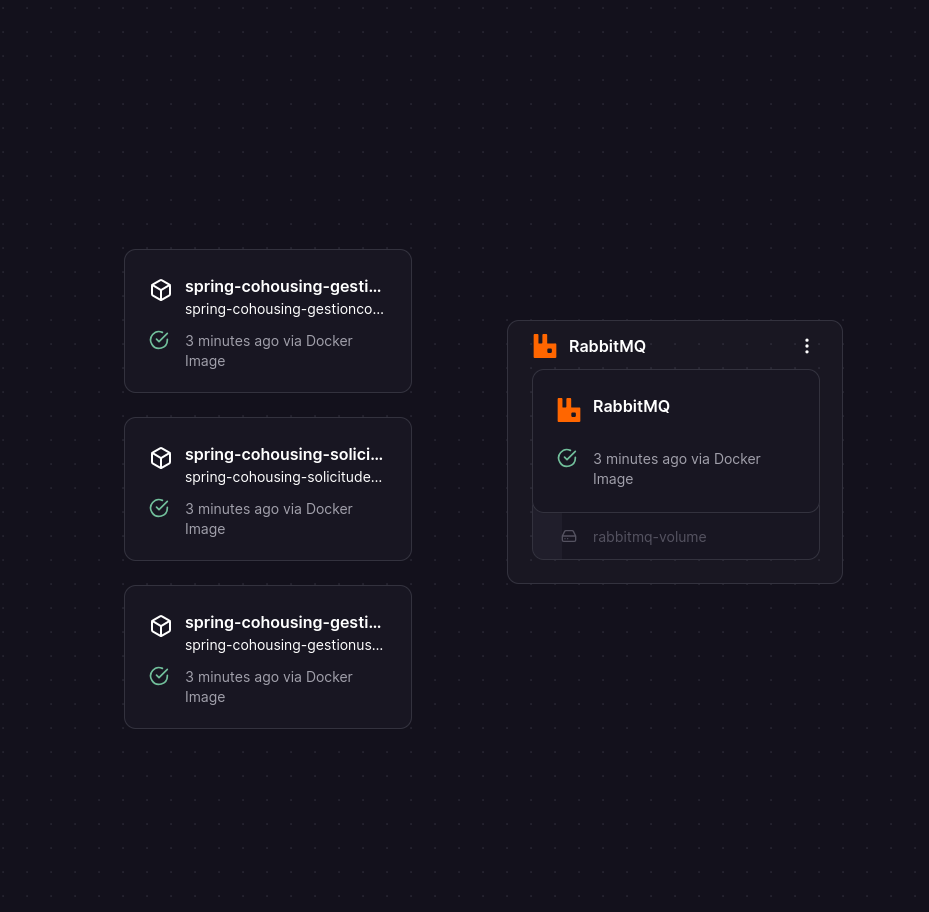
\includegraphics[width=1\textwidth]{fotos/railway2.png}
  \caption{Muestra del tablero de despliegue del segundo proyecto en Railway}
  \label{fig:railway2}
\end{figure}
Cada microservicio ha sido desplegado en \textbf{Railway} a partir de su respectivo Dockerfile subido a DockerHub, estos han ido actualizándose cada vez que se realizaba un \textbf{merge} a la rama \texttt{main} (producción). Además, se ha configurado una serie de variables para cada servicio, de forma que puedan conectarse con las bases de datos y con el servicio de Rabbitmq. Estas variables son inyectadas automáticamente en el código a partir de un archivo \texttt{application-prod.properties} y un perfil activo \texttt{prod}.

En cuanto a la seguridad, tanto Railway como GitHub Pages proporcionan URLs para cada servicio con \textbf{HTTPS}, lo que garantiza que el tráfico entre el cliente y los servicios esté cifrado, evitando el envío en texto plano.

\vspace{0.5em}
Los servicios desplegados en Railway han sido los siguientes:
\vspace{0.5em}
\begin{itemize} \item \textbf{Microservicio de Gestión de Usuarios}: \href{https://spring-cohousing-GestionUsuarios-production.up.railway.app}{spring-cohousing-GestionUsuarios-production.up.railway.app} \vspace{0.25em} \item \textbf{Microservicio de Gestión de Comunidades}: \href{https://spring-cohousing-GestionComunidades-production.up.railway.app}{spring-cohousing-GestionComunidades-production.up.railway.app} \vspace{0.25em} \item \textbf{Microservicio Recomendador}: \href{https://python-cohousing-recomendador-production.up.railway.app}{python-cohousing-recomendador-production.up.railway.app} \vspace{0.25em} \item \textbf{Microservicio de Solicitudes}: \href{https://spring-cohousing-Solicitudes-production.up.railway.app}{spring-cohousing-Solicitudes-production.up.railway.app} \vspace{0.25em} \item \textbf{Bases de datos}: Tres bases de datos PostgreSQL denominadas \texttt{Postgres-Comunidad}, \texttt{Postgres-Usuarios} y \texttt{Postgres-Solicitudes} \vspace{0.25em} \item \textbf{Microservicio ApiGateway}: \href{https://spring-cohousing-apigateaway-production.up.railway.app}{spring-cohousing-apigateaway-production.up.railway.app} \vspace{0.25em} \item \textbf{Servicio RabbitMQ}: Desplegado a partir de una plantilla obtenida en DockerHub. \end{itemize}


\vspace{0.5em}


    \chapter{Conclusiones} \label{diseño}

En este último capítulo se presenta un análisis de las conclusiones del proyecto realizado. Para ello, se realizará un balance general de los objetivos planteados y de su completitud durante el transcurso del proyecto. Además, se incluirá una reflexión sobre el impacto que este trabajo ha tenido en mi formación y sobre cómo las habilidades obtenidas se podrán aplicar en el desarrollo de una carrera como Ingeniero de Software. Finalmente, se comentarán posibles trabajos a futuro orientados a mejorar la aplicación desarrollada.

\section{Balance general}
Tras los meses de trabajo en el desarrollo del proyecto, \textbf{ShareSpace}, se ha logrado estructurar un sistema completo de \textbf{microservicios}, garantizando tanto la resiliencia frente a errores como la escalabilidad. Además, se ha diseñado un \textbf{frontend} que permite al usuario interactuar con la aplicación de manera intuitiva. Todo el desarrollo ha sido complementado con un \textbf{flujo completo de CI/CD} mediante \textbf{GitHub Actions}. Finalmente, se ha realizado un despliegue real utilizando las plataformas \textbf{GitHub Pages} y \textbf{Railway} \cite{Railway}. Todo ello ha permitido crear una solución al problema inicial planteado, asegurando la calidad y aplicando técnicas de desarrollo de software actuales.

\subsection{Objetivos conseguidos}

En primer lugar, se logró establecer una metodología de trabajo basada en Scrum, adaptada al carácter individual de un TFG. Se identificaron las tareas a implementar en la aplicación, se crearon historias de usuario a partir de ellas, se agruparon en iteraciones y se organizaron en un diagrama de Gantt. Todo ello quedó reflejado en \textbf{GitHub}, garantizando que el desarrollo del software estuviese estrechamente ligado a la planificación del proyecto.  

Se ha conseguido integrar \textbf{GitHub} de forma central durante todo el desarrollo. No solo se reflejaron las historias de usuario junto a las iteraciones a las que pertenecen en GitHub Project, sino que las tres ramas principales del repositorio han guiado el flujo de desarrollo de la funcionalidad. Además, las \textbf{GitHub Actions}, como herramienta de \textbf{CI/CD}, han contribuido a mejorar la calidad y fiabilidad del código, siendo parte esencial del flujo completo del desarrollo.

Tecnológicamente, se ha logrado profundizar en herramientas actuales presentes en entornos profesionales, como \textbf{Docker} y \textbf{Docker Compose} para la contenedorización, \textbf{Spring Boot} para el backend y \textbf{React} con \textbf{TypeScript} para el frontend. Asimismo, se ha comprendido el diseño completo de una arquitectura compleja basada en microservicios, identificando responsabilidades de cada servicio, implementado \textbf{comunicación asíncrona} entre microservicios mediante \textbf{Rabbitmq}, y desarrollando componentes esenciales como el \textbf{API Gateway}.

A nivel de desarrollo, se ha conseguido asegurar la calidad del código, profundizando en el uso de patrones de diseño y arquitecturas limpias.

Finalmente, se ha podido realizar un despliegue completo del sistema utilizando \textbf{Railway}, una herramienta que ha permitido desplegar el Dockerfile de cada microservicio subido a \textbf{Docker Hub}, así como el servicio de \textbf{Rabbitmq} y las bases de datos. Con esto se ha concluido el desarrollo completo del proyecto, desde la creación de las bases hasta su despliegue en la nube.

\section{Valoración final}

Tras la realización de este proyecto, se ha proporcionado una solución al problema identificado, creando una propuesta final que ofrece una experiencia completa al usuario.

Desde el punto de vista académico, este trabajo ha supuesto una oportunidad para aplicar de forma práctica los conocimientos adquiridos a lo largo del grado, especialmente en asignaturas vinculadas a la mención de Ingeniería del Software. Asignaturas como \textit{Metodología de Desarrollo Ágil} (MDA) o \textit{Desarrollo y Gestión de Proyectos} (DGP) han resultado fundamentales para planificar y organizar el proyecto mediante la metodología ágil SCRUM, permitiendo estructurar adecuadamente las tareas, la planificación temporal y la entrega iterativa de versiones.

Desde una perspectiva personal, me siento orgulloso del resultado obtenido. Este proyecto nació de una necesidad real que me afectaba personalmente y ha sido desarrollado desde cero con una visión profesional. No se ha tratado únicamente de programar, sino de diseñar y tomar decisiones técnicas justificadas, poniendo al usuario en el centro del proceso. Cada aspecto del desarrollo ha seguido principios sólidos de ingeniería del software, incorporando herramientas y prácticas comunes en el mundo profesional, como el uso de contenedores, GitHub, CI/CD y despliegue automatizado.

Considero que todo lo aprendido y aplicado en este proyecto se puede trasladar al ámbito profesional, donde es imprescindible entender cómo estructurar la lógica de negocio de una propuesta y cómo aplicar una arquitectura en consecuencia. Al analizar ofertas de trabajo en el sector, se puede observar que muchas de las competencias demandadas por las empresas han sido puestas en práctica a lo largo de este trabajo.

\section{Trabajos Futuros}

Con el objetivo de ampliar y mejorar el proyecto desarrollado, se han identificado y analizado una serie de mejoras que podrían integrarse en la aplicación para optimizar la experiencia del usuario. A continuación, se exponen las más representativas:

\begin{itemize}
    \item \textbf{Integrar un sistema de chat}: Permitiría a los usuarios comunicarse directamente con los administradores antes de solicitar la unión a una comunidad, resolviendo dudas previas y acercando a los usuarios buscadores a los ofertantes.
    \item \textbf{Desarrollar una versión móvil}: Ofrecer una versión adaptada para dispositivos móviles. Usando tecnologías como React Native, se podría adaptar gran parte del código actual del frontend a un formato móvil.
    \item \textbf{Automatizar el despliegue móvil}: Implementar una GitHub Action que automatice el despliegue de la versión móvil. Una vez desarrollado, se podría incluir en el CI/CD para que la aplicación evolucione a medida que se desarrolla funcionalidad.
    \item \textbf{Solicitudes en tiempo real}: Crear un sistema de notificaciones basado en WebSocket para permitir la actualización en tiempo real. Esto permitiría mostrar las solicitudes que tiene pendiente el usuario en tiempo real, pudiendo añadir un indicador que muestre el número actualizado de pendientes.
    \item \textbf{Pruebas de rendimiento}: Realizar pruebas de rendimiento para evaluar cómo responde cada microservicio bajo distintas cargas en escenarios reales de uso, comprobando la eficiencia y respuesta del sistema.
    \item \textbf{Refuerzo de la seguridad}: Mejorar la seguridad en el almacenamiento de datos para proteger la información de los usuarios.
    \item \textbf{Publicar en plataformas oficiales}: Desplegar la aplicación móvil en plataformas oficiales, como App Store, permitiendo su acceso a un mayor volumen de usuarios.
\end{itemize}

\vspace{0.5em}
Las mejoras propuestas se centran principalmente en ofrecer una solución móvil que permita a los usuarios disfrutar de una experiencia de calidad. Para ello, será necesario adaptar el código a React Native o alguna plataforma similar. Además, la implementación de WebSocket para las solicitudes supondría una mejora significativa en la interacción y usabilidad para el usuario. Personalmente, me gustaría continuar con las mejoras de la aplicación, ya que su implementación podría suponer un gran aprendizaje.

    
	\newpage
	\bibliography{bibliografia}
	\bibliographystyle{plain}

	\newpage


\end{document}

